\chapter{Rapid prototyping of parameterized acoustofluidic microchannels towards isolation of bacteria for point of care diagnostics}
\label{chapter:acoust}
\thispagestyle{myheadings}

% set this to the location of the figures for this chapter. it may
% also want to be ../Figures/2_Body/ or something. make sure that
% it has a trailing directory separator (i.e., '/')!
\graphicspath{{4_acoust/Figures/}}

\section{Introduction}
\label{sec:acoust_intro}
Acoustic manipulation has emerged as a versatile method for microfluidic separation and concentration of particles and cells. It has advantages over other methods because of high throughput, no affinity chemistry, and no electrodes or specialized structures in the microchannel.  The efficiency of the separation depends only on microchannel dimensions appropriately selected for the ultrasonic excitation frequency. However, the potential of plastic acoustofluidic devices is hampered by complex boundary conditions relative to those of more rigid materials, ultimately resulting in the lack of a predictive model. In the absence of a mechanism for predicting focusing conditions, improvements in device performance must either be delayed indefinitely until a model is built or one must experimentally explore a seemingly unbounded solution space dictated by non-continuous, non-linear performance patterns. In the absence of a rapid prototyping framework, the latter choice can involve prohibitive amounts of time and fabrication costs and thus is not a practical option. This paper presents such a framework and uses it to explore the complex, multi-dimensional response surface ultimately arriving at a device geometry better able to separate bacteria from clinical blood samples to downstream biochemical reactions that result in an optical read out.  This detector uses a proprietary synthetic biology approach to optically identify target pathogens and rapidly test their susceptibility to antibiotics.

\section{Problem Statment}
\label{sec:acoust_ps}
Silicon, glass, or metal devices are commonly used for acoustophoresis because the rigid channel walls provide a near ideal acoustic boundary against the sample fluid, enhancing the required standing wave resonance \cite{laurell2007chip}.  This ideal boundary simplifies design because the resultant reduction in mathematical complexity allows for the development of models that can be used to calculate the resonant modes in the channel-fluid system \cite{petersson2007free}.  However, the rigid materials previously used are expensive and slow to manufacture, have poor compatibility with many biological samples, and are unlikely to be acceptable for mass production of disposable laboratory tools \cite{nge2013advances}.  Recent work has demonstrated acceptable levels of acoustic separation in plastic, showing that acoustic separation is possible in polystyrene, opening the door to low-cost diagnostic and therapeutic devices \cite{mueller2013continuous}.

To further optimize acoustic microfluidics in plastic in the absence of a predictive model, an experimental investigation is needed.  While acoustic separation in plastic is proven to work experimentally, enhancing performance is challenging because the simplified analysis developed by others no longer applies, since the channel walls can no longer be considered ideally rigid \cite{barnkob2010measuring}. Additionally, while plastic acoustofluidic devices can be scaled using methods such as hot embossing or injection molding \cite{koerner2005epoxy}, prototyping geometries in small batches remains an expensive proposition. 

This study seeks to find a better-performing device geometry when compared to the device currently in use, which will be referred to as the \textit{baseline}. Fabrication costs will be minimized by manufacturing chips on-site through the use of an automated, rapid prototyping software framework in conjunction with a new class of inexpensive, desktop computer numerical controlled (CNC) micromills. Devices were screened in rapid succession using a performance parameter described in Section \ref{sec:img} while varying two measures of merit, dissipated power and volumetric flow rate, towards enhancing the separation performance of point-of-care plastic acoustofluidic devices.

\section{Methods}
\label{sec:methods}

\begin{figure}[htb]
  \begin{minipage}[t]{0.99\linewidth}\centering
    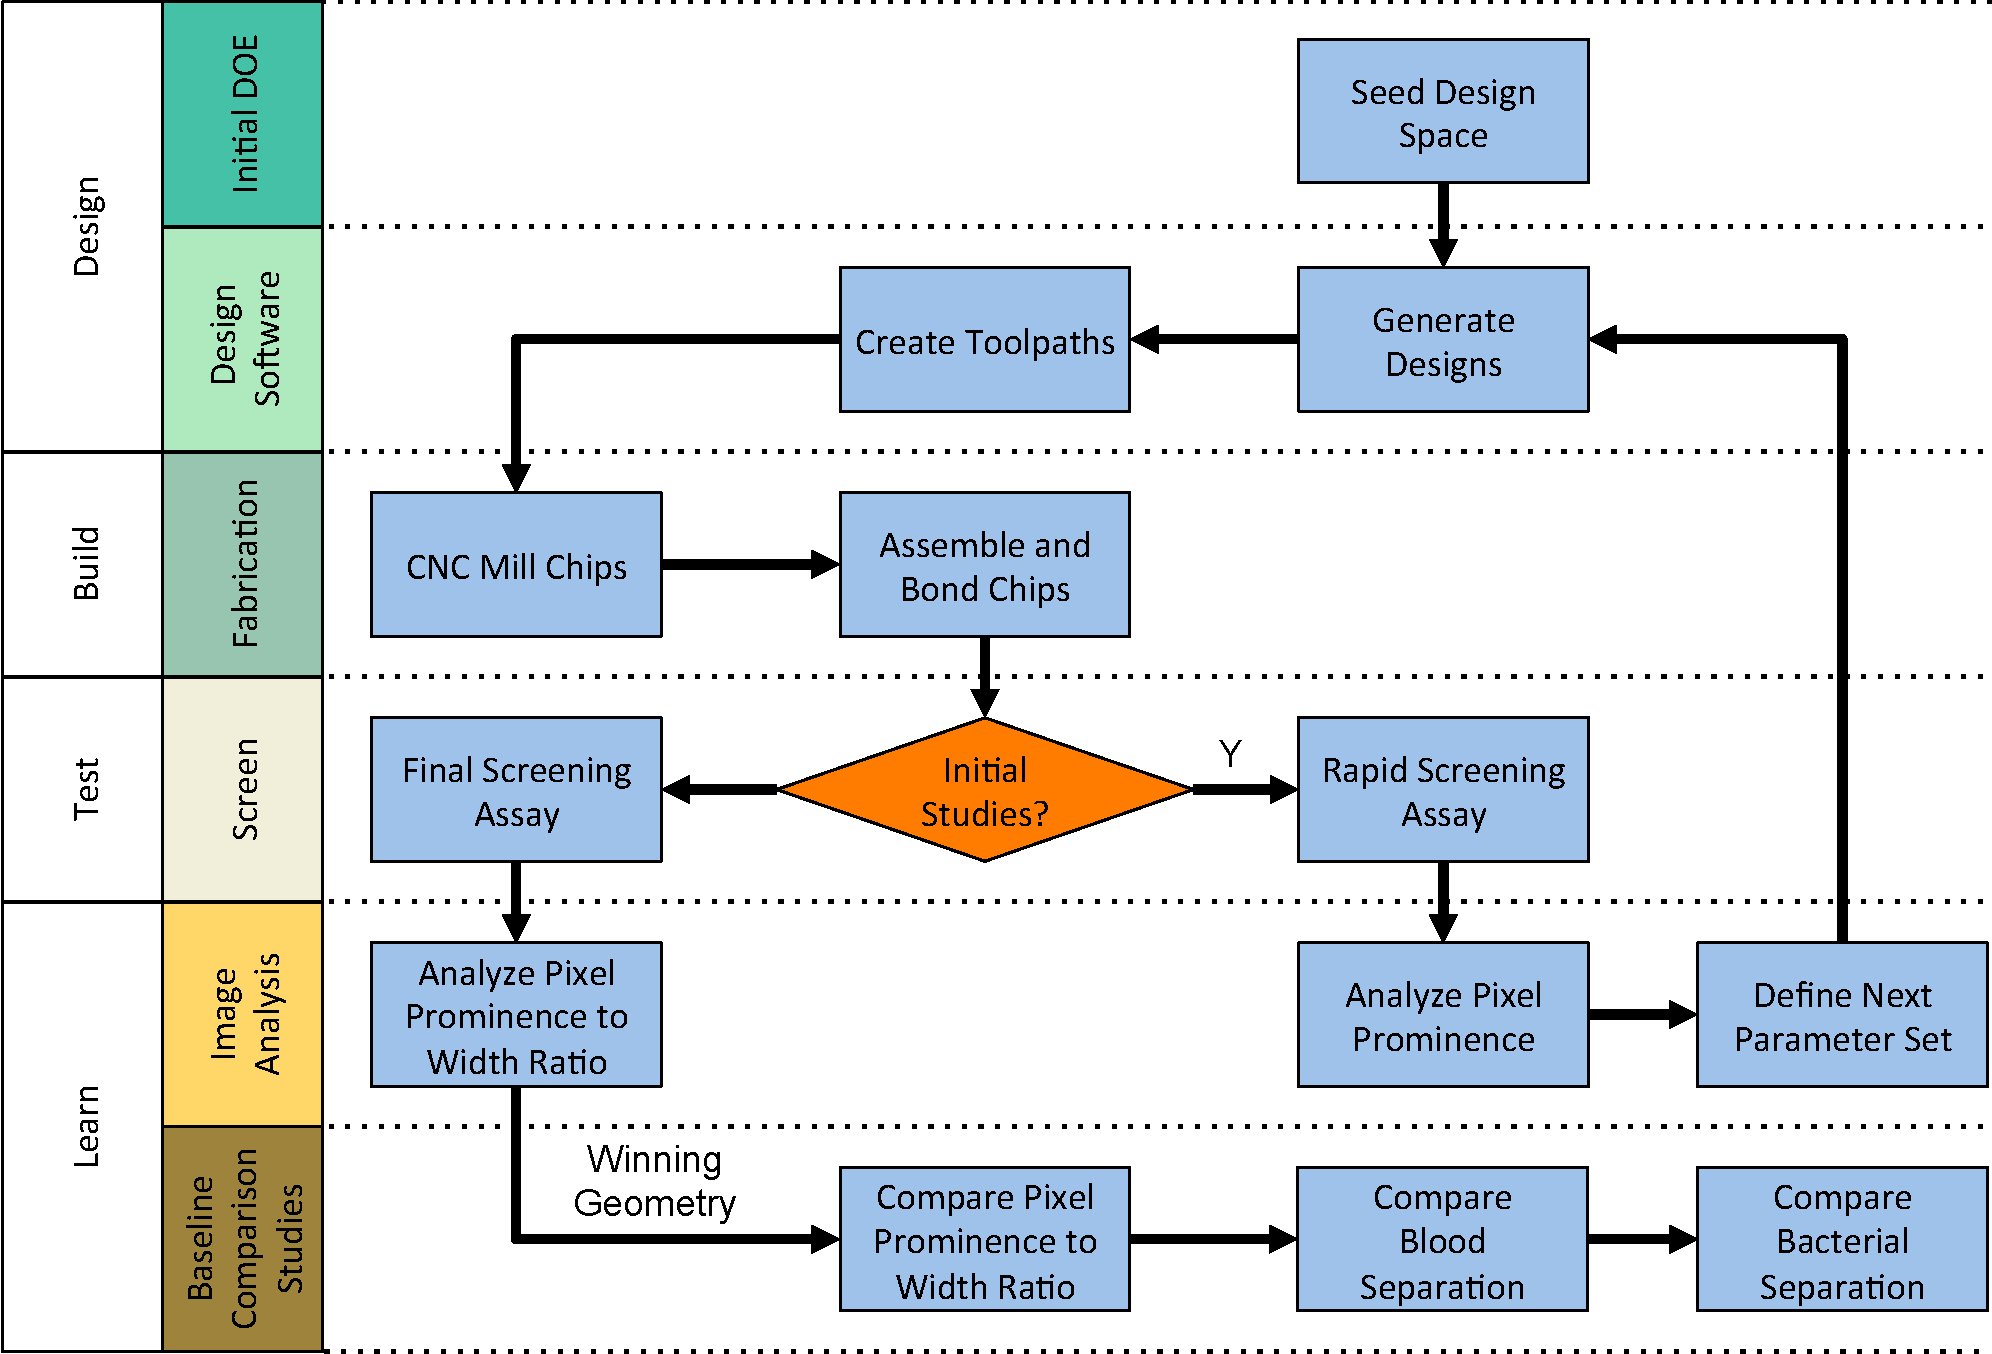
\includegraphics[width=14cm]{flow.pdf}
  \end{minipage}\hfill
\caption{Rapid Prototyping Workflow.}
\label{fig:flow}       % Give a unique label
\end{figure}

%Section \ref{ssec:seeding} describe the initial seeding of the design space using an orthogonal array of four geometric parameters, each having three levels. Chips are then designed, fabricated and assembled using methods described in Section \ref{sec:rp}. A rapid screening assay is performed on this initial design set.

Figure \ref{fig:flow} illustrates the iterative workflow used in conducting the study. The basic theory of operation for the acoustofluidic separation device is explained in Section \ref{sec:chipDesign}. Section \ref{sec:rp} summarizes the methods used to design and manufacture new chip geometries. Section \ref{sec:experiment} defines the two types of assays used in the screening phase of the workflow as well as the blood and bacterial separation experiments used to compare the performance of the new geometry to that of the baseline. Section \ref{sec:img} outlines the methodology used to screen separation performance from microscope images. Finally, Section \ref{sec:results} presents the results of the device screening as well as the winning design's performance when compared to that of the baseline geometry. 

\section{Chip Design and Theory of Operation}
\label{sec:chipDesign}

\textbf{TODO Jason: Help here please!}\\

Figure \ref{fig:geometry}a. is a top-down, two-dimensional drawing of the trifurcated acoustic separation device. The device functions by focusing large particles, such as red blood cells (RBCs) and white blood cells (WBCs), to the center port, while smaller particles (ex., platelets, bacteria, etc.) are collected at the side port. This trifurcated device is used in the blood and bacterial separation experiments described in Section \ref{ssec:comparison}. In order to reduce manufacturing complexity, devices screened using the methods outlined in Section \ref{ssec:screen} consist only of the input port; fluid channel, defined as the channel upstream of the trifurcation; and a single output port. The cross-sectional geometries, defined in Figure \ref{fig:geometry}b., apply to this simplified device design. 

\begin{figure}[htb]
  \begin{minipage}[t]{0.99\linewidth}\centering
    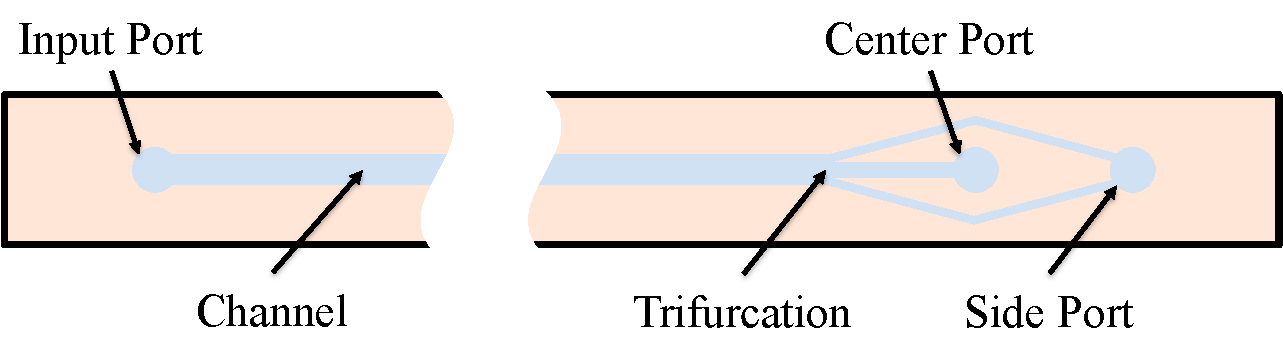
\includegraphics[width=14cm]{chip}
    \medskip
    \centerline{(a)}
  \end{minipage}\hfill\\
  \begin{minipage}[t]{0.99\linewidth}\centering
    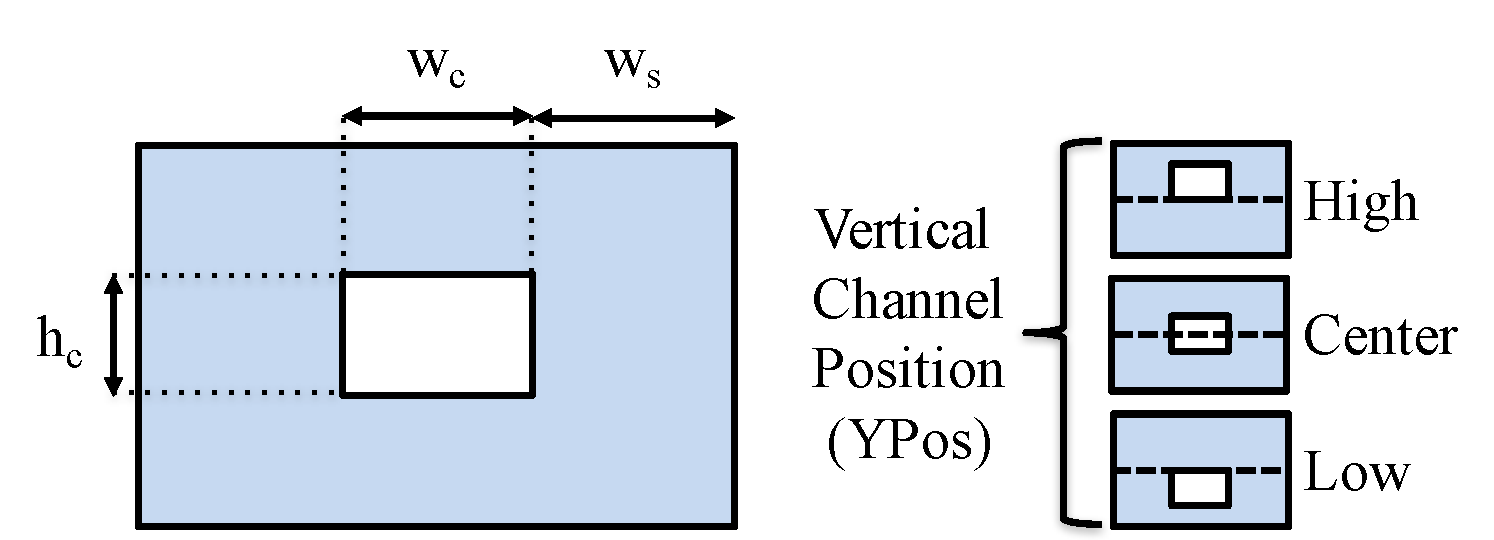
\includegraphics[width=14cm]{2D}
    \medskip
    \centerline{(b)}
  \end{minipage}
  \caption[Acoustofluidic separation device and 2D geometric definitions]{(a) Complete trifurcated microfluidic separation chip. (b) Definitions for each two-dimensional geometry included in the study. Note that the definitions apply to fluidic channel upstream of the trifurcation.}
  \label{fig:geometry}
\end{figure}

\section{Rapid Prototyping}
\label{sec:rp}
The success of this study relied upon the ability to quickly design and fabricate iterations of chip geometries. Previous design optimization efforts were hampered by the process of out-sourcing device fabrication. Each design iteration required a fully specified mechanical drawing and any changes to the design demanded regeneration of the solid model. Once the drawing for a single design iteration was prepared and submitted to a machine shop lead times in excess of two weeks were not uncommon while costs soared as high as \$3,000 for a batch of 20 identical chips. This section describes how these limitations were mitigated using free and open-source design software in conjunction with a \$2,500 desktop micromill.

\subsection{Design Generation}
\label{ssec:design}
Three levels of software are required to design and fabricate a novel chip geometry using a Computer Numerical Control (CNC) micromill. A Computer Aided Design (CAD) tool is used to create a solid model of the device. Second, Computer Aided Manufacturing (CAM) software is responsible for generating the commands (also called toolpaths) that are sent directly to the micromill. Finally, a piece of control software is required to manage the connection between a computer and the micromill. This software sends individual toolpath commands from the computer to the micromill. 

Device designs were created using OpenSCAD \cite{wikiOpenScad}, a free and open source CAD tool that reads script files to generate solid models. A custom library was used to create solid models using just the geometric parameters outlined in Figure \ref{fig:geometry}b. as inputs. Figure \ref{fig:listing1} shows the solid model for a single device design created using the function call in Listing \ref{lst:chip}. Figure \ref{fig:layout} shows how an array of distinct solid models can be created from a few lines of code shown in Listing \ref{lst:chipLayout}. This array of designs is spaced according the size of the endmill used by the CNC to cut out each design, thus allowing for seamless processing by CAM software (Autodesk Fusion 360).

\begin{minipage}{0.99\linewidth}
\begin{lstlisting}[caption={The custom OpenSCAD library allows solid model creation using just a single line of code},label={lst:chip}, frame=single, language=scad]
  chip(Wc=0.55,Hc=0.25,Ws=0.85,YPos=high);
\end{lstlisting}
\end{minipage}

\begin{figure}[htb]
  \begin{minipage}[t]{0.99\linewidth}\centering
    
\includegraphics[width=14cm]{PaperExampleListing1}
  \end{minipage}\hfill
  \caption[Single solid geometry]{Output solid geometry of Listing 1, including bonding plate.}
  \label{fig:listing1}
\end{figure}


\begin{minipage}{0.99\linewidth}
\begin{lstlisting}[caption={The single line of code in Listing \ref{lst:chip} can then be iterated upon to form an array of different device geometries that can be sent directly to a CAM tool for toolpath generation}, label={lst:chipLayout}, frame=single, language=scad]
include<chip.scad>

wc=[1.5,1,0.5];
ws=[0.5,1.5,2.5];
hc=[0.1,0.2,0.25];
ypos=[high,high,high];
Spacing=0.79375;         //End Mill Diameter

numChips=len(wc);

module chipLayout(){
  for(i=[0:(numChips-1)]){
    let (ChipY=wc[i]+ws[i]*2){
      translate([0,2*i*(ChipY+Spacing),0])
      chip(Wc=wc[i],Hc=hc[i],Ws=ws[i],YPos=ypos[i]);
    }
  }
}
\end{lstlisting}
\end{minipage}

\begin{figure}[htb]
  \begin{minipage}[t]{0.99\linewidth}\centering
    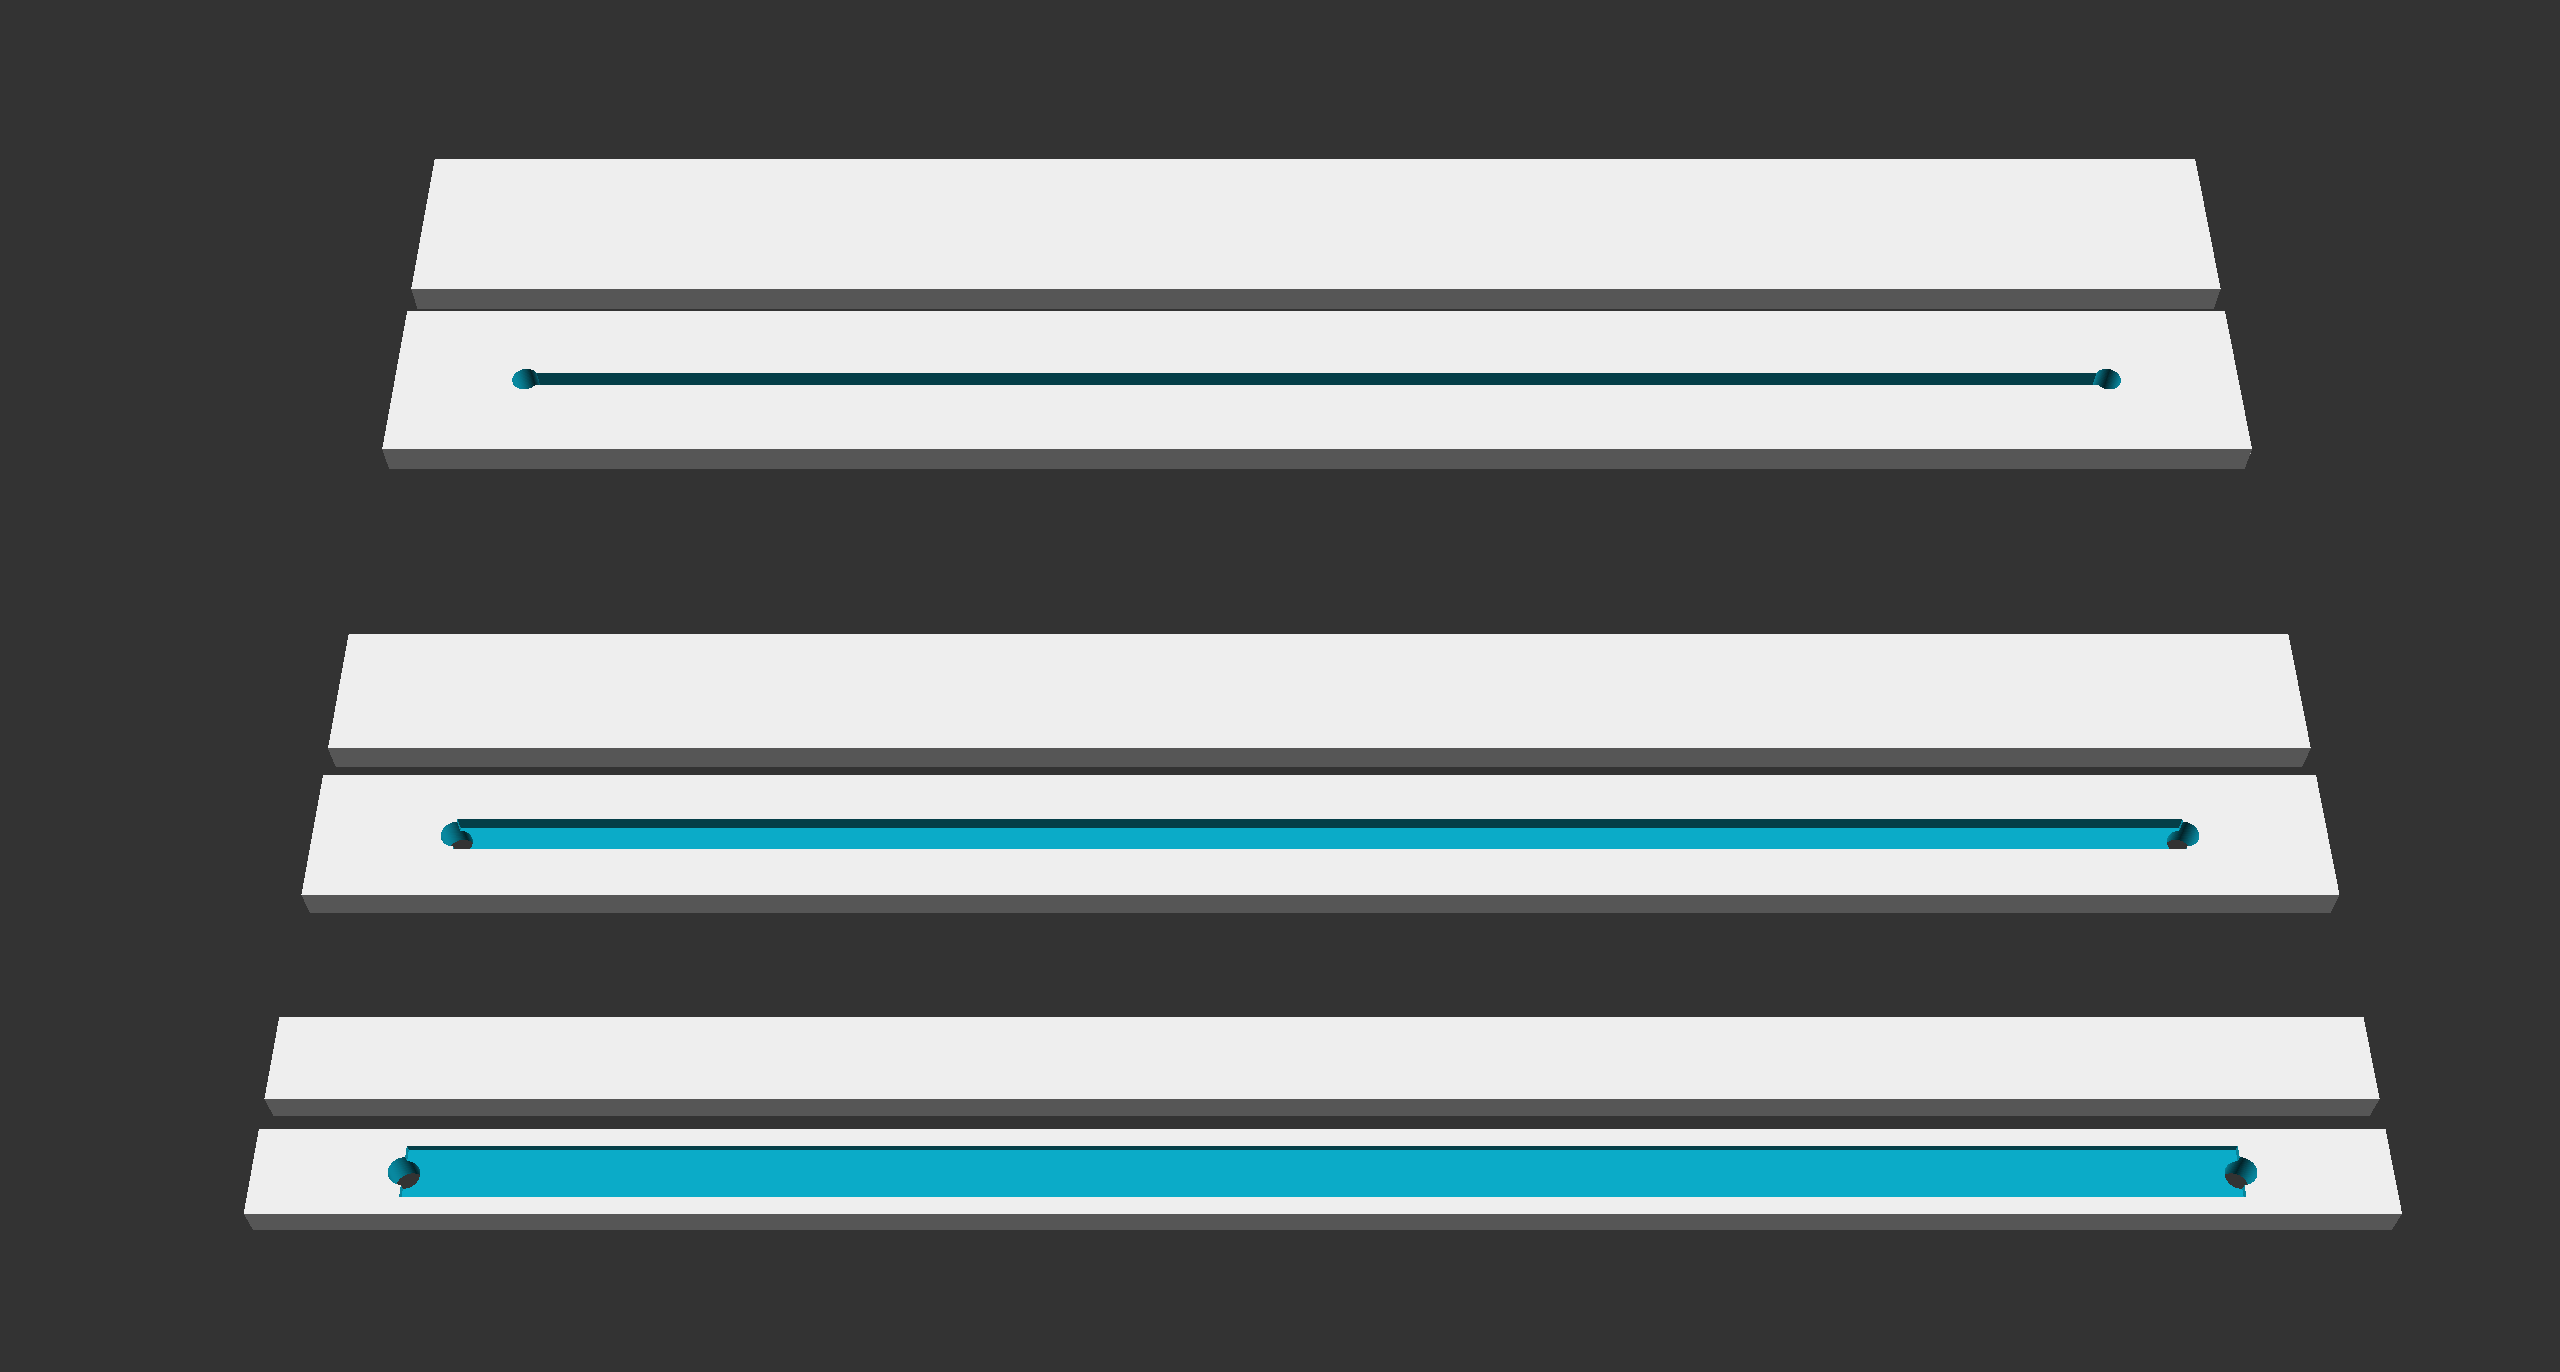
\includegraphics[width=14cm]{ExampleLayout}
  \end{minipage}\hfill
  \caption[Example layout of multiple device designs]{Output solid geometry of Listing 2, which includes three different designs and their corresponding bonding plates.}
	\label{fig:layout}
\end{figure}


\subsection{Fabrication}
\label{ssec:fab}

Micromilling has demonstrated potential for prototyping plastic microfluidic devices in terms of time and cost when compared to other fabrication methods such as embossing and injection molding \cite{guckenberger2015micromilling}. While such studies claim that micromilling devices using an outside source can lower costs to \$137 per batch and 11-15 days of turn-around time, these costs only consider material costs and not labor, which can drive up the cost of prototyping an order of magnitude \cite{guckenberger2015micromilling}. Costs per device can be lowered to less than \$1 if devices can be fabricated in-house; however, the costs associated with establishing such capabilities can be staggering. Micromills capable of achieving resolutions at or below 25 $\mu$m start at \$15k. The large footprints and noise associated with these machines can make them inappropriate for use within a microfluidics laboratory. Self-contained micromills drive costs up another order of magnitude. Additionally, the cost in terms of expertise required to operate a micromill is non-trivial. The software stack associated with generating toolpaths for a micromill does not currently resemble the simplicity of other CNC machines such as 3D printers, which only require a solid model generated from a CAD tool, such as SolidWorks, and a slicer which can generate toolpaths with a minimal amount of user input. Micromilling requires a suite of CAM tools that demand extensive knowledge of various tooling strategies such as feed rate, depth of cut and spindle speed that vary with each material and tool size. 

Recent advances in micromilling has led to the formation of a new class of desktop micromills, which can offer 25 $\mu$m resolution at costs starting at \$2,500 all in a form-factor appropriate for a typical laboratory bench \cite{yen2016cost}. While these new machines still require knowledge of CAD and CAM software tools, research in automation techniques specifically for micromilling microfluidics is beginning to bear fruit \cite{silva2016iwbda}. This study leverages these advancements to quickly manufacture distinct acoustofluidic device designs at a negligible cost when compared to outsourcing fabrication.

\subsection{Materials and Assembly}
Polystyrene (PS) was selected as an appropriate material based on its low attenuation and high impedance of ultrasonic energy \cite{wang2001high}. The chip was sealed using a thermal bonding method previously described \cite{mueller2013continuous}. 0.75'' lengths of Polyetheretherketone (PEEK) tubing served as an interface between the PS chip and the longer lengths of polyvinyl chloride (PVC) tubing used to introduce and collect sample. The rigid PEEK tubing was inserted into machined port cavities and affixed to the chip using epoxy (Epoxy 907, Miller-Stephenson, Danbury, CT, USA). 

The sealed chip was mounted to a lead zirconate titanate (PZT) transducer (APC International, PZT 850) with a published resonance of 2.34 MHz using low viscosity cyanoacrylate adhesive.  


\section{Experimental Methodology}
\label{sec:experiment}
This study required four types of experiments: rapid screening, final screening, blood separation and bacterial separation. Rapid screening assays were conducted on two initial parameter sets labeled as ``Initial Studies'' in Figure \ref{fig:flow}. The methodology for this assay is outlined in Section \ref{sssec:rapidScreen} and the initial parameter sets upon which this assay were conducted are defined in Sections \ref{ssec:seeding} and \ref{sssec:width}. The results of these two initial rapid screening assays were used to inform the parameter set of a final, more involved, screening assay described in Section \ref{sssec:finalScreen} and the parameter set upon which this study was conducted is defined in Section \ref{sssec:height}. 

Ultimately, the performance of the final screening assay's winning geometry was compared to that of the baseline geometry in three different experiments measuring a device's ability to focus blood using a quantitative visual inspection, focus blood by measuring RBC concentration in the center port, as well as separate bacteria from whole blood. Performance was scored based on parameters defined for each experiment. Later experiments (i.e., after rapid screening) measured a device's efficacy while minimizing dissipated power and maximizing throughput (i.e., volumetric flow rate). These measures of merit are fully defined in Section \ref{ssec:MoM}.

\subsection{Measures of Merit}
\label{ssec:MoM}

%The two measures of merit used in this study are average dissipated power of the transducer and volumetric flow rate of a clinical sample. Minimizing the transducer's power requirement via a geometry with an optimized resonance profile is desirable as high power requirements can result in localized heat buildup and chip failure. Maximizing volumetric flow rate allows for more rapid sample enrichment.

%\textbf{TODO Charlie: Add verbiage as to why we use Power as a measure of merit (tie displacement to power)}

The two measures of merit used in this study are the volumetric flow rate and the average electrical power. Maximizing the volumetric flow rate will enable the largest volume of input sample to be enriched in the shortest amount of time. This is typically favorable in most diagnostic and therapeutic applications, as long as performance (i.e., enrichment of sample) is not reduced considerably. In this study, the volumetric flow rate through a device under test was regulated by a syringe pump (PhD Ultra, Harvard Apparatus). Minimizing the power requirements of the system is another important measure of merit which has multiple implications. First, heat generated in the transducer and in the PS channel during actuation may lead to delamination of the channel or may be harmful to the clinical sample. Therefore, it is best to drive the system at the smallest amplitude necessary to achieve acceptable performance. Second, if better performance can be achieved at lower power levels, this may enable an increase in the volumetric flow rate. We quantify dissipated power as described in section \ref{sssec:power} below.

\subsubsection{Volumetric Flow Rate}

The volumetric flow rate, measured in $\mu$l/min, through a device under test was regulated by a syringe pump (PhD Ultra, Harvard Apparatus).

\textbf{\\TODO: Anything else to say about flow rate? If not, then this need not be a numbered section}

\subsubsection{Average Dissipated Power}
\label{sssec:power}

The sinusoidal signal used to drive the transducer is generated by a function generator (AFG3022C, Tektronix, Beaverton, OR, USA) and amplified using a broadband RF amplifier (AG1021, T\&C Power Conversion, Rochester, NY, USA). The instantaneous voltage and current across the transducer is monitored using an oscilloscope (DPO2024B, Tektronix, Beaverton, OR, USA). In order to determine the actual power consumed by the transducer, it is first necessary to consider the instantaneous power as follows:

\begin{equation}
\label{eqn:instpower}
\hfill P_{inst} = VI = V_{max}sin(\omega t) I_{max} sin(\omega t-\varphi),\hfill
\end{equation}

\noindent where $V_{max}$ and $I_{max}$ are the maximum values of voltage and current, $\varphi$ is the phase lag between the instantaneous current and voltage signals, and $\omega=2\pi f$ is the sinusoidal drive frequency in rad/s. Using trigonometric identities and integrating over a cycle of the sinusoid we compute the average consumed power as:

\begin{equation}
\label{eqn:avgpower}
\hfill P_{avg} = V_{rms}I_{rms}cos\varphi,\hfill
\end{equation}

\noindent where $V_{rms}$ and $I_{rms}$ are the root mean square values of voltage and current. Using the oscilloscope, we multiply the instantaneous voltage and current and compute the average of this product to find the average consumed power in real time throughout our experiments.
\subsection{Blood Sample Preparation}
All experiments in this study used human whole blood (Interstate Labs) anticoagulated with acid–citrate–dextrose. In each case, the blood was diluted to 5\% hematocrit in phosphate buffer solution (PBS 7.4 pH Lot Number 1832496). Cellular concentrations were measured before and after dilution using an automated hematology analyzer (Sysmex XXX). The diluted sample was then transferred to a 10 mL syringe (BD 10 mL Luer-Lok tip syringe 309604) and introduced to the chip through PVC tubing. 

\subsection{Screening Assays}
\label{ssec:screen}
Two types screening assays were conducted, both of which analyzed device performance through the use of microscope images and derived pixel intensities as a surrogate for focusing performance. This method is based on the assumption that higher concentrations of red blood cells will appear visibly darker, and hence have a higher grayscale value, when better acoustic focusing is present. This assumption is based on observations shown in Figures \ref{fig:pixelPerformance} and \ref{fig:microscopePics}, which demonstrate that in conditions conducive to good focusing (ex., lower flow rate and higher dissipated power) the observable band of blood cells will appear narrower and darker and thus have a correspondingly higher grayscale value within this band. Data confirming this assumption is presented in Section \ref{sssec:comparisonBlood}, which measures the relative RBC concentrations between the center and side ports of the trifurcated chip design.

\begin{figure}[htb]
  \begin{minipage}[t]{0.49\linewidth}\centering
    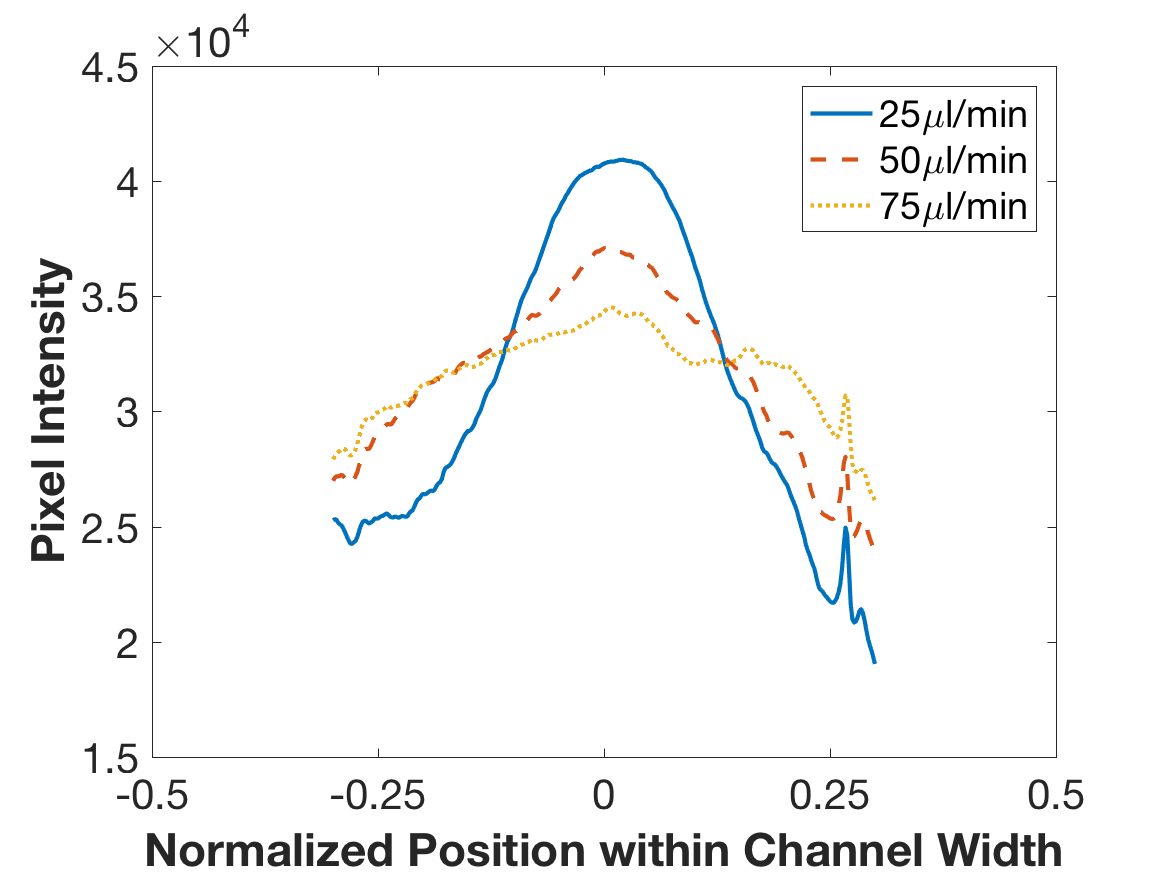
\includegraphics[width=7cm]{Baseline3PromFlow}
    \medskip
    \centerline{(a)}
  \end{minipage}\hfill
  \begin{minipage}[t]{0.49\linewidth}\centering
    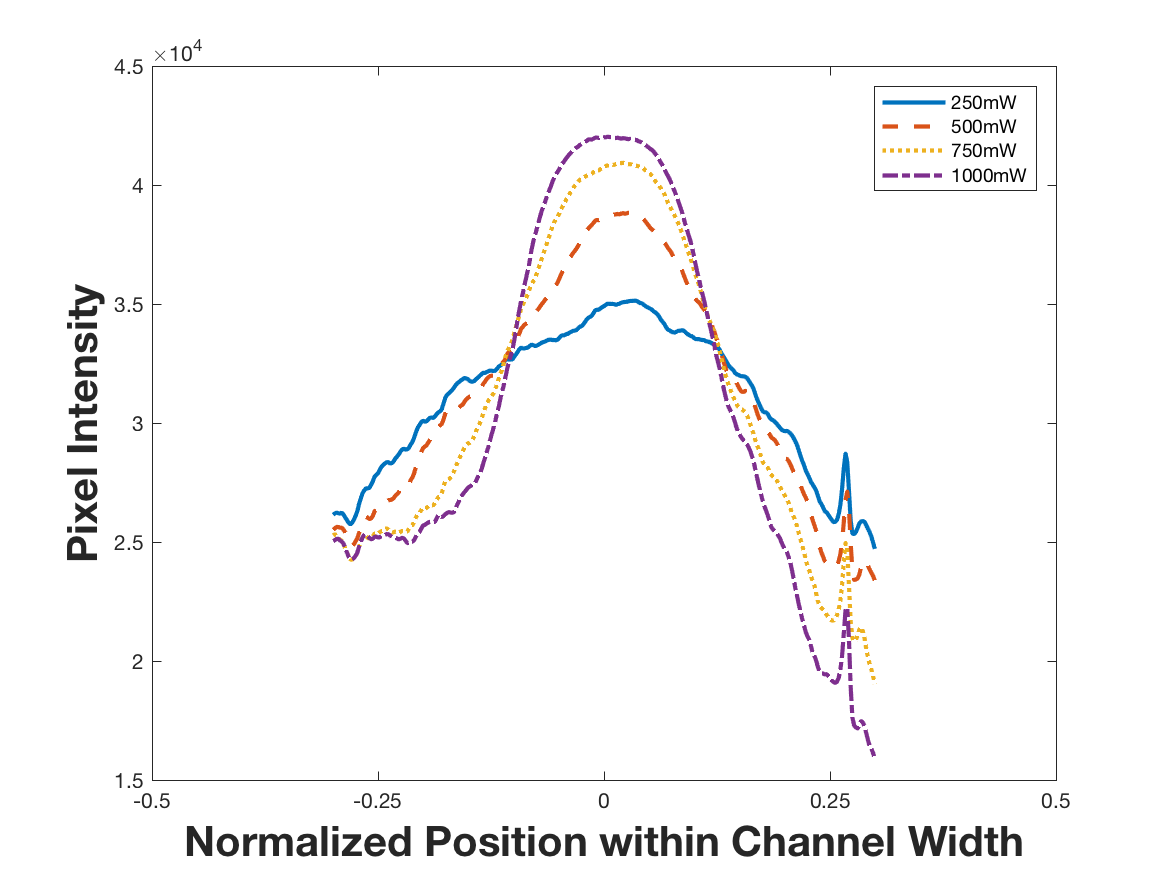
\includegraphics[width=7cm]{Baseline3PromPower}
    \medskip
    \centerline{(b)}
  \end{minipage}
  \caption[Pixel grayscale values across the width of the fluidic channel]{Pixel grayscale values across the width of the fluidic channel. (a) Power is held constant at 750mW, while flow rate is varied. (b) Flow rate is held constant at 25ul/min, while power is varied. Note that maximum pixel intensity, and thus focusing performance, increases as flow rate is decreased.}
	\label{fig:pixelPerformance}
\end{figure}

\begin{figure}[htb]
  \begin{minipage}[t]{0.49\linewidth}\centering
    
\includegraphics[width=7cm]{25ul250mWBaseline_3}
    \medskip
    \centerline{(a)}
  \end{minipage}\hfill
  \begin{minipage}[t]{0.49\linewidth}\centering
    
\includegraphics[width=7cm]{25ul500mWBaseline_3}
    \medskip
    \centerline{(b)}
  \end{minipage}\\
  \begin{minipage}[t]{0.49\linewidth}\centering
    
\includegraphics[width=7cm]{25ul750mWBaseline_3}
    \medskip
    \centerline{(c)}
  \end{minipage}\hfill
  \begin{minipage}[t]{0.49\linewidth}\centering
    
\includegraphics[width=7cm]{25ul1000mWBaseline_3}
    \medskip
    \centerline{(d)}
  \end{minipage}\\
  \caption[Microscope images at resonant frequency for increasing power levels]{Microscope images of focusing performance at resonant frequency with increasing power at levels of 250mW (a), 500mW (b), 750mW (c), 1000mW (d). The plots in Figure \ref{fig:pixelPerformance}(b) are derived directly from these images.}
	\label{fig:microscopePics}
\end{figure}

The two types of screening assays, rapid screening and final screening, each have different assumptions regarding the nature of their input parameter sets. The rapid screening assay does not make any assumptions regarding the functionality of a device under test. This means that it is reasonable to assume that a device will not exhibit acoustic focusing at any frequency within the tested bandwidth under the experimental conditions; thus, the performance parameter by which devices are scored seeks to determine the existence of acoustic focusing, rather than discern the relative quality of focusing between devices. The performance parameter used in this case is called \emph{prominence} and is defined in Section \ref{ssec:prom}. 

In contrast, the final screening assay attempts to compare the relative performance of devices that are assumed to exhibit some acceptable measure of focusing performance. Devices are scored based on the ratio of prominence to the width of the focusing band, as defined in Section \ref{ssec:promToWidth}. The relative merits between the two performance parameters are discussed in Section \ref{sec:img}. 

\subsubsection{Rapid Screening Assay}
\label{sssec:rapidScreen}

The purpose of the rapid screening assay was to discover functional device designs, i.e., designs that could focus blood, and the frequencies at which they operate. This was accomplished by testing many devices under the same power and flow conditions while sweeping through a frequency band around which the baseline geometry operates while remaining below the piezoelectric transducer's resonant frequency. The flow rate was set such that the particle velocity of each chip design was normalized to that of the baseline device operating at a flow rate of 100 $\mu$l/min. The input power was normalized by setting the average dissipated power to 1 W at 1 MHz, the operating frequency of the baseline geometry, and then maintaining this input power throughout the frequency sweep.

Taking into account the operating frequency of the baseline device (1 MHz) as well as the resonant frequency of the transducer (2.34 MHz), the chosen frequency band spanned from 0.50 -- 2.00 MHz, inclusive. Within this frequency band pictures were taken in 10 kHz increments, from which a number corresponding to the maximum peak prominence was returned. The maximum peak prominence for the entire frequency band constituted the score for that particular design.

\subsubsection{Final Screening Assay}
\label{sssec:finalScreen}

The final screening assay served to discriminate between devices of assumed functionality. This was accomplished by manually tuning the device to its operating frequency and then modulating the measures of merit. Three flow rates (25 $\mu$l/min, 50 $\mu$l/min, and 75 $\mu$l/min) and four power levels (250 mW, 500 mW, 750 mW, and 1000 mW) were studied. A microscope image was captured for each combination of flow rate and power level, from which the ratio of peak prominence to width was calculated in accordance with the method described in Section \ref{ssec:promToWidth}.

\subsection{Blood Separation Assay}
\label{ssec:bloodAssay}

Due to differences between side and center channel outlet dimensions at the point of trifurcation, outlet tubing length was cut to match the ratio of hydrolic diameters of each channel. Once flow fractions matched outlet dimensions, the channel was primed with deionized (DI) water, followed by the sample.  Once the sample being tested occupied the total volume of the microfluidic chip and inlet/outlet tubing, the flow rate was set to appropriate setting on the syringe pump.  Control measurements were taken for each flow rate with the acoustics off to validate flow fraction as well as cellular behavior within microfluidic chip.  Samples were collected in conical tubes and measured for flow fraction and cell quantity calculations. The resonant frequency was found visually by observing the focusing stream - the most compact stream reveals the resonant frequency.  Once the resonant frequency was found, powers were swept by increasing RF amplifier gain to encompass the experimental parameters.  For each sample, weights and hematology data was taken and entered into a database.  MATLAB was used for further data analysis and plotting.

\subsection{Bacterial Separation Assay}
\label{ssec:bacteriaAssay}

\textbf{TODO Parker: Please fill in this section with a paragraph describing the experimental conditions for the plating experiment}

\begin{figure}[htb]
  \begin{minipage}[t]{0.99\linewidth}\centering
    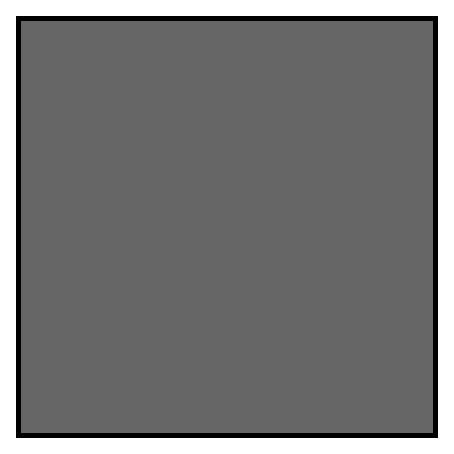
\includegraphics[width=12cm]{example}
  \end{minipage}\hfill
	\caption{Render of the experimental setup including custom stage, piezoelectric transducer and microfluidic chip.}
	\label{fig:setup}
\end{figure}

\section{Image Analysis}
\label{sec:img}
Image processing software (ImageJ \cite{imagej}) was used to create a plot profile of pixel intensities across the width of the channel, $W_c$. Devices were screened using the prominence of local maxima, as defined in Section \ref{ssec:prom}, as a performance parameter. Prominence has advantages over raw pixel intensity for the purposes of comparison due to its self-normalizing nature. Since prominence is measured relative to points on the signal itself it is robust against irregularities inherent to the signal. These irregularities can take the form of variable lighting conditions between experimental runs, such as variations in environmental lighting, and illumination variabilities within a single microscope image's region of interest, such as skewed background intensities caused by shadows. 

Peak prominence is used as a direct measure of merit for device screening studies in which the assumption of a functional geometry (i.e. a geometry capable of focusing particles) cannot be made. When a device is determined to function well based on its prominence score it is compared to the baseline geometry using the ratio of peak prominence to half-prominence width, $\chi$ (Figure \ref{fig:algProg}c.). $\chi$ cannot be used during device screening as the metric can skew results by rewarding peaks with relatively small prominence values and correspondingly small widths. However, this metric is useful for comparing the quality of the most prominent peaks among different, commensurate, devices such as the winner of a design screening iteration and the baseline geometry.

Once a device compares favorably against the baseline in terms of $\chi$, this final design's separation performance is then tested head-to-head against the baseline geometry using the full, trifurcated, designs shown in Figure \ref{fig:geometry}(a). by comparing each design's ability to focus blood to the center channel, as shown in Figure \ref{fig:geometry}, as well as each design's ability to separate bacteria from blood. These experiments are described in further detail in Section \ref{ssec:comparison}.

\subsection{Definition of Prominence}
\label{ssec:prom}
Suppose an ordered signal is defined as in Equation \ref{eqn:sig}, where set $D$ consists of $N$ data points. Prominence is calculated by first finding all local maxima within the response set $D$ and then determining a reference point on the signal associated with each local maxima \cite{arge2013algorithms}. Briefly, this reference point is established by drawing a horizontal line in both the positive and negative directions from the local maxima until either the end of the signal is reached or until the line intersects the signal itself, thus creating two sets of data points in the positive and negative directions. Minima are determined for each of the data sets, and prominence is then defined as the height of the local maxima relative to the maximum of these two established minima. 

\begin{equation}
  \label{eqn:sig}
  \hfill s[n]=D \quad n=0,1,2,\cdots,N-1 \hfill
\end{equation}

A framework for defining prominence in a more formal terms begins by establishing the data structure for the signal of interest. Individual values are accessed by index such that $s[i]=d_i, d_i\in D$. Two discrete points $d_i \in D$ and $d_{i'} \in D$ are said to be $neighbors$ if $|i-i'| = 1$. A local maxima, hereafter called a $peak$, is a point $p$ where $d_i$ is greater than all of its neighbors, as defined in Algorithm \ref{alg:peaks}. The set of peaks $P \subset D$ consists of individual peak values $p \in P$. A peak is referenced by its index value $i$ in $D$ and the raw peak height is calculated by finding $s[i]$. The index in $D$ of peak $p$ is returned by the function $x(p)$. The height of peak $p$ is returned by the function $s[x(p)]$. Thus if $p \leftarrow d_i$, $x(p)=i$ and $s[x(p)]=d_i$. Prominence is then determined via Algorithm \ref{alg:prom}. 

%\paragraph{Paragraph headings} Use paragraph headings as needed.
%\begin{equation}
%a^2+b^2=c^2
%\end{equation}

\begin{figure}
\begin{algorithm}[H]
\DontPrintSemicolon
\SetKwFunction{AppendToP}{AppendToP}
\SetKwData{neighbors}{neighbors}
\KwData{Ordered data set $D$}
\KwResult{A list of peaks $P\subset D$}
\Begin{
$P \longleftarrow \emptyset$\;
\For{$d_i \in D$}{
    Find all $neighbors$ for $d_i \mid |i-i'|=1$
    $\AppendToP(neighbors)$
}
}
\caption{Find Peaks. Finds all local maxima in $D$ and returns them as a list of peaks $P$ as shown in Figure \ref{fig:algProg}(a). \label{alg:peaks}}
\end{algorithm}
\end{figure}

\begin{figure}
\begin{algorithm}[H]
\DontPrintSemicolon
\SetKwData{s_{low}}{s_{low}}
\SetKwFunction{AppendToWidth}{AppendToWidth}
\KwData{Ordered data set $D$ and a list of local maxima $P\subset D$}
\KwResult{A list of prominence values, $Prom$, for each local maxima, $p$}
\Begin{
$Prom \longleftarrow \emptyset$\;
  \For{$p_j \in P$}{
	\tcc{Scan Low}
	\For{$i = 0$ to $x(p_j)$}{
	  \If{$x(p_j)=0$}{
	    $i_{low}=x(p_j)$\;
	    Exit Loop\;
	  }
	  \ElseIf{$s[x(p_j)-i] \geq s[x(p_j)] \lor x(p_j)-i=0$}{
	    $i_{low}=x(p_j)-i$\;
	    Exit Loop\;
	  }
	}
	\For{$i = 0$ to $N-1$}{
	  \If{$x(p_j)=N-1$}{
	    $i_{high}=x(p_j)$\;
	    Exit Loop\;
	  }
	  \ElseIf{$s[x(p_j)+i] \geq s[x(p_j)] \lor x(p_j)+i=N-1$}{
	    $i_{high}=x(p_j)+i$\;
	    Exit Loop\;
	  }
	}
  $s_{low}=min(s[i_{low}] \to s[x(p_j)])$\;
  $s_{high}=min(s[x(p_j)] \to s[i_{high}])$\;
  $s_{ref}=max(s_{low},s_{high})$\;
  $Prom_j = s[x(p_j)] - s_{ref}$\;
  $\AppendToWidth(Prom_j)$\;
  }
}
\caption{\label{alg:prom}Calculate Prominence. Draw a horizontal line to the left (low) and right (high) of the peak until the end of the signal is reached or until the signal is intersected. Record the indices of each as $i_{low}$ and $i_{high}$, respectively. Find the minima in each set and use the maximum of the minima to set the reference level. Calculate a peak's prominence by subtracting the reference level from the raw signal value of the peak (Figure \ref{fig:algProg}(b-c))}
\end{algorithm}
\end{figure}

\subsection{Definition of Prominence to Width Ratio, $\chi$}
\label{ssec:promToWidth}
The half-prominence width of a peak of prominence $Prom$ is calculated by drawing two horizontal lines extending in the negative and positive directions from the point of half-prominence. These lines extend in either direction until either the end of the signal is reached or the line intersects the signal itself. The indices of these events in the negative and positive directions are recorded as $i^-$ and $i^+$, respectively. The peak width $HalfPromWidth$ is then defined as $|i^+-i^-|$. It has been shown that for equivalent focusing performance, the prominence scales with the channel width \cite{ley2016continuum}, therefore it is appropriate to normalize the peak width by the width of the channel. The final equation for $\chi$ is shown in Equation \ref{eqn:ratio}

\begin{figure}
\begin{algorithm}[H]
\DontPrintSemicolon
\SetKwData{s_{low}}{s_{low}}
\SetKwFunction{FindPeaks}{FindPeaks}
\KwData{A list of prominence values, $Prom$, for each local maxima, $p$}
\KwResult{A list of half-prominence peak widths $HalfPromWidth$, for each local maxima, $p$}
\Begin{
$Prom \longleftarrow \emptyset$\;
  \For{$p_k \in P$}{
	\tcc{Scan Left}
	\For{$i = 0$ to $x(p_k)$}{
	  \If{$x(p_k)=0$}{
	    $i^-=x(p_k)$\;
	    Exit Loop\;
	  }
	  \ElseIf{$s[x(p_k)-i] \leq s[x(p_k)]-\frac{Prom_k}{2} \lor x(p_k)-i=0$}{
	    $i^-=x(p_k)-i$\;
	    Exit Loop\;
	  }
	}
	\tcc{Scan Right}
	\For{$i = 0$ to $N-1$}{
	  \If{$x(p_k)=N-1$}{
	    $i^+=x(p_k)$\;
	    Exit Loop\;
	  }
	  \ElseIf{$s[x(p_k)+i] \leq s[x(p_k)]-\frac{Prom_k}{2} \lor x(p_k)+i=N-1$}{
	    $i^+=x(p_k)+i$\;
	    Exit Loop\;
	  }
	}
  $HalfPromWidth_k = i^+-i^-$\;
  $\AppendToWidth(HalfPromWidth_k)$\;
  }
}
\caption{\label{alg:width}Calculate Peak Width at Half Prominence. Draw a horizontal line to the left (-) and right (+) at the median of the prominence line until either the end of the signal is reached or until the signal is intersected. Record the indices of each as $i^{-}$ and $i^{+}$, respectively. The absolute value of the difference between these index values is the peak width at half prominence. \ref{fig:algProg}(d))}
\end{algorithm}
\end{figure}

\begin{equation}
\label{eqn:ratio}
\hfill \chi=Prom*\frac{W_c}{HalfPromWidth}\hfill
\end{equation}

\begin{figure}[htb]
  \begin{minipage}[t]{0.49\linewidth}\centering
    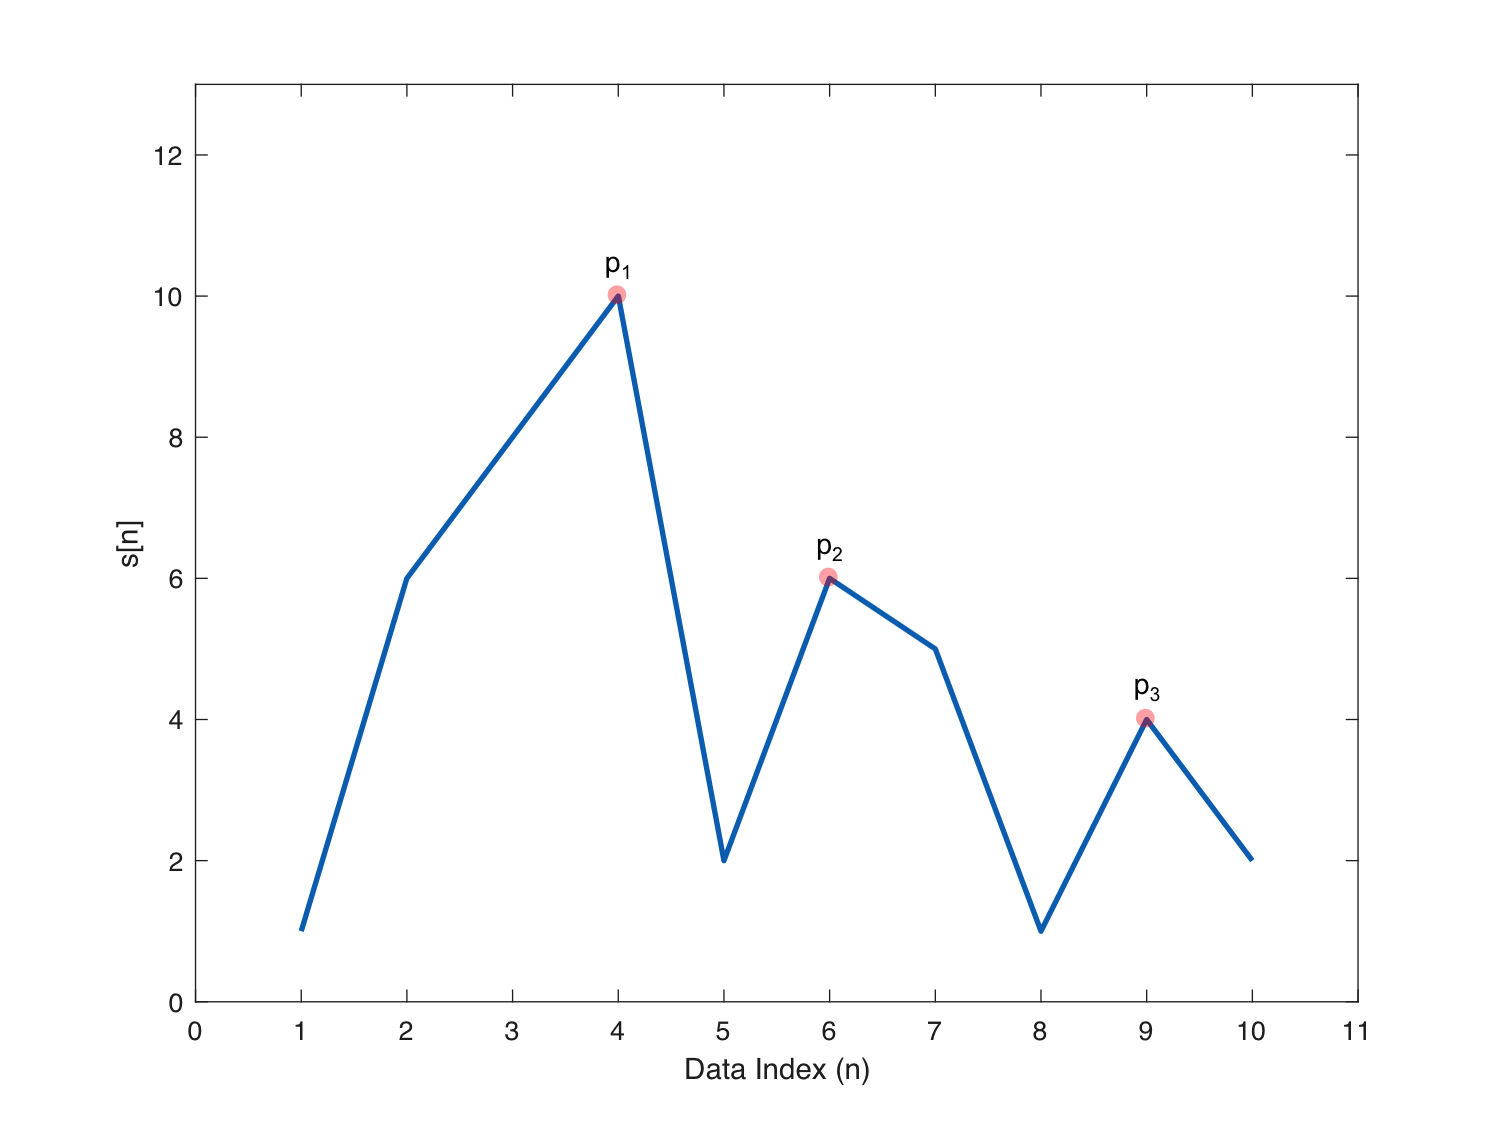
\includegraphics[width=7cm]{localMax}
    \medskip
    \centerline{(a)}
  \end{minipage}\hfill
  \begin{minipage}[t]{0.49\linewidth}\centering
    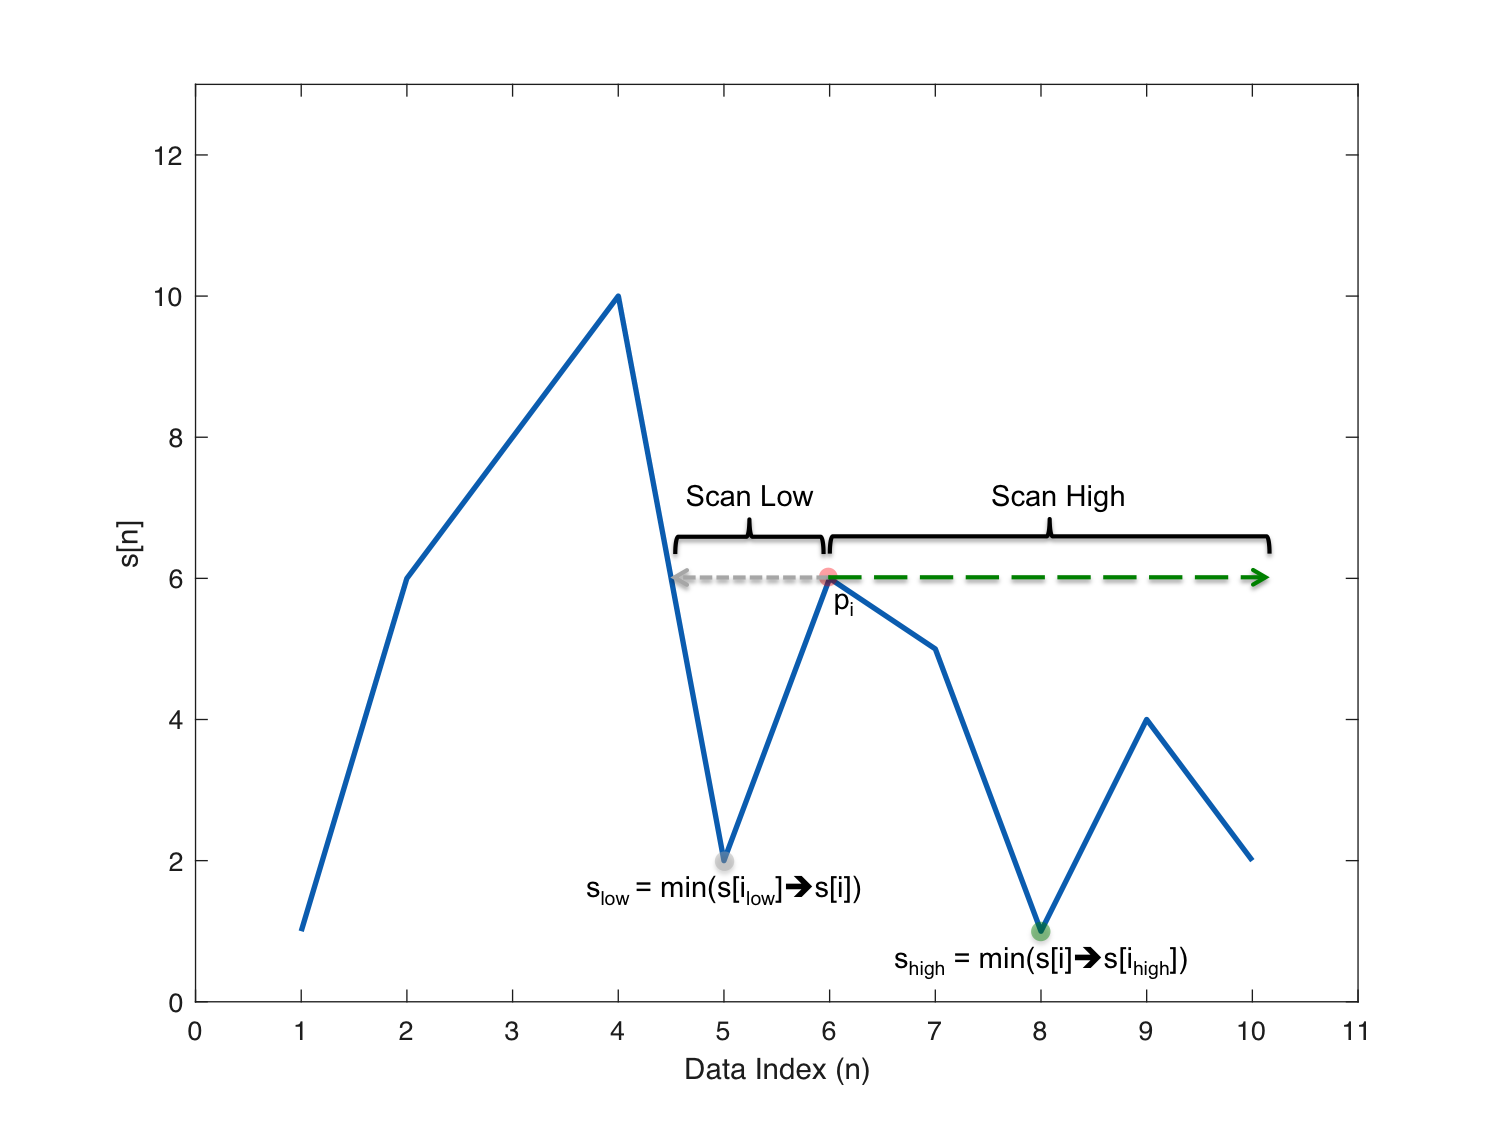
\includegraphics[width=7cm]{scan}
    \medskip
    \centerline{(b)}
  \end{minipage}\\
  \begin{minipage}[t]{0.49\linewidth}\centering
    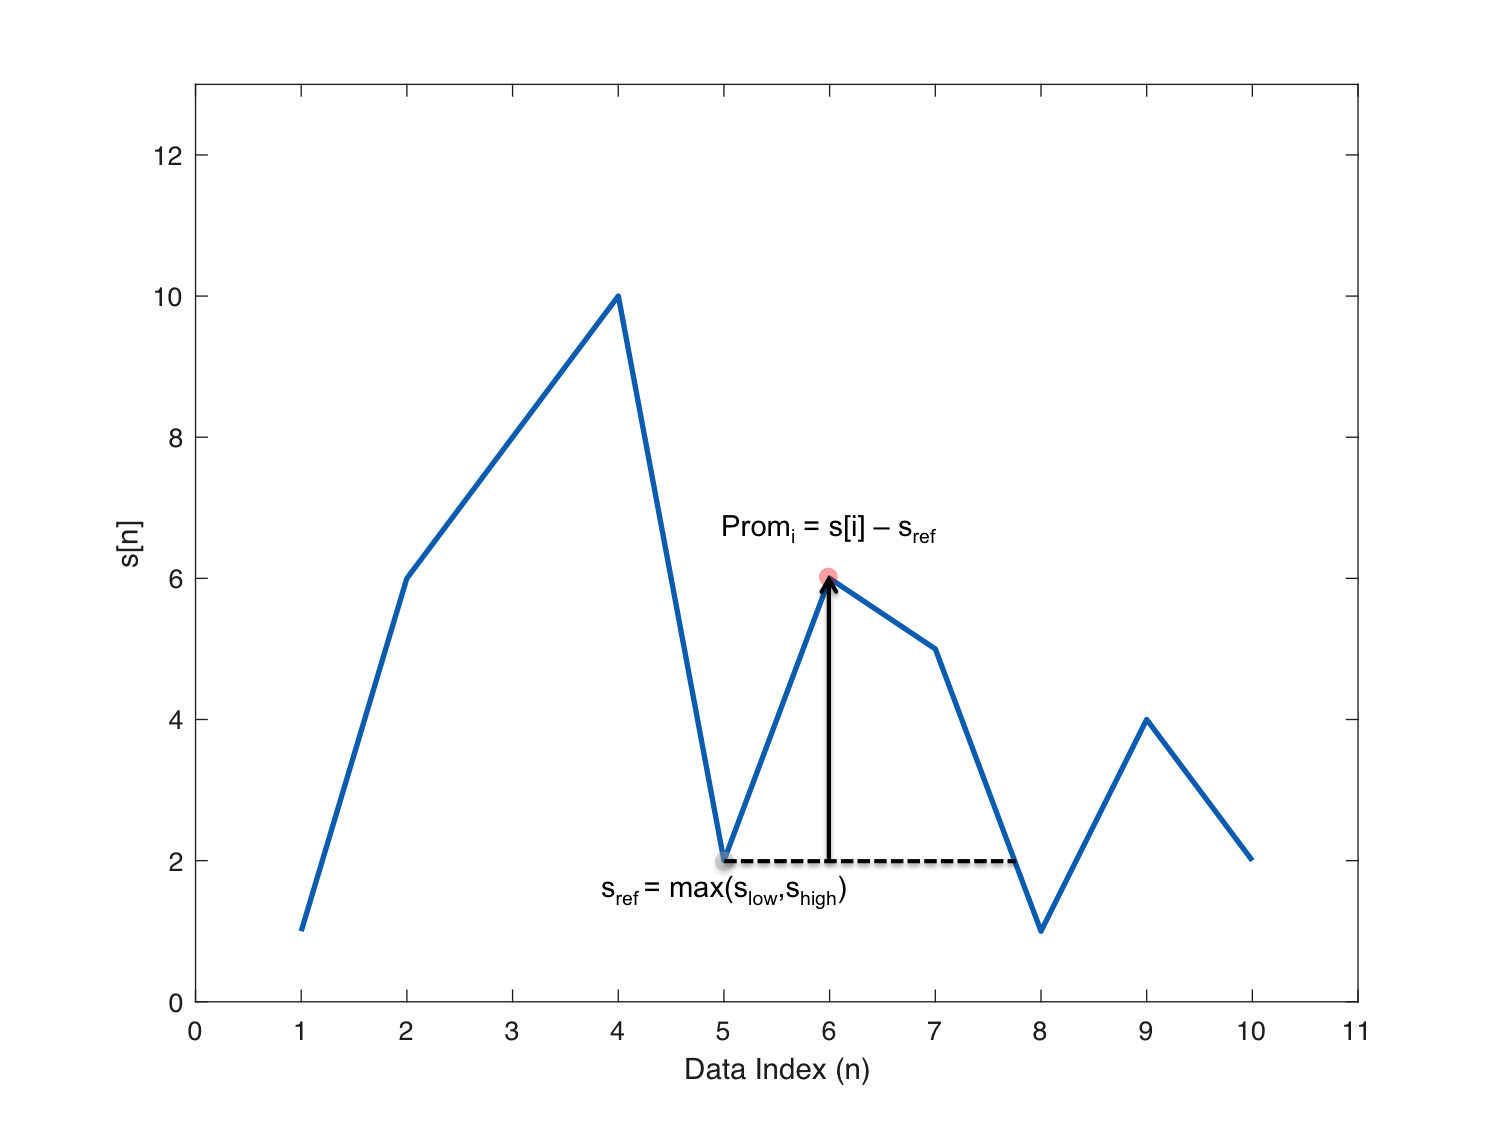
\includegraphics[width=7cm]{calcProm}
    \medskip
    \centerline{(c)}
  \end{minipage}\hfill
  \begin{minipage}[t]{0.49\linewidth}\centering
    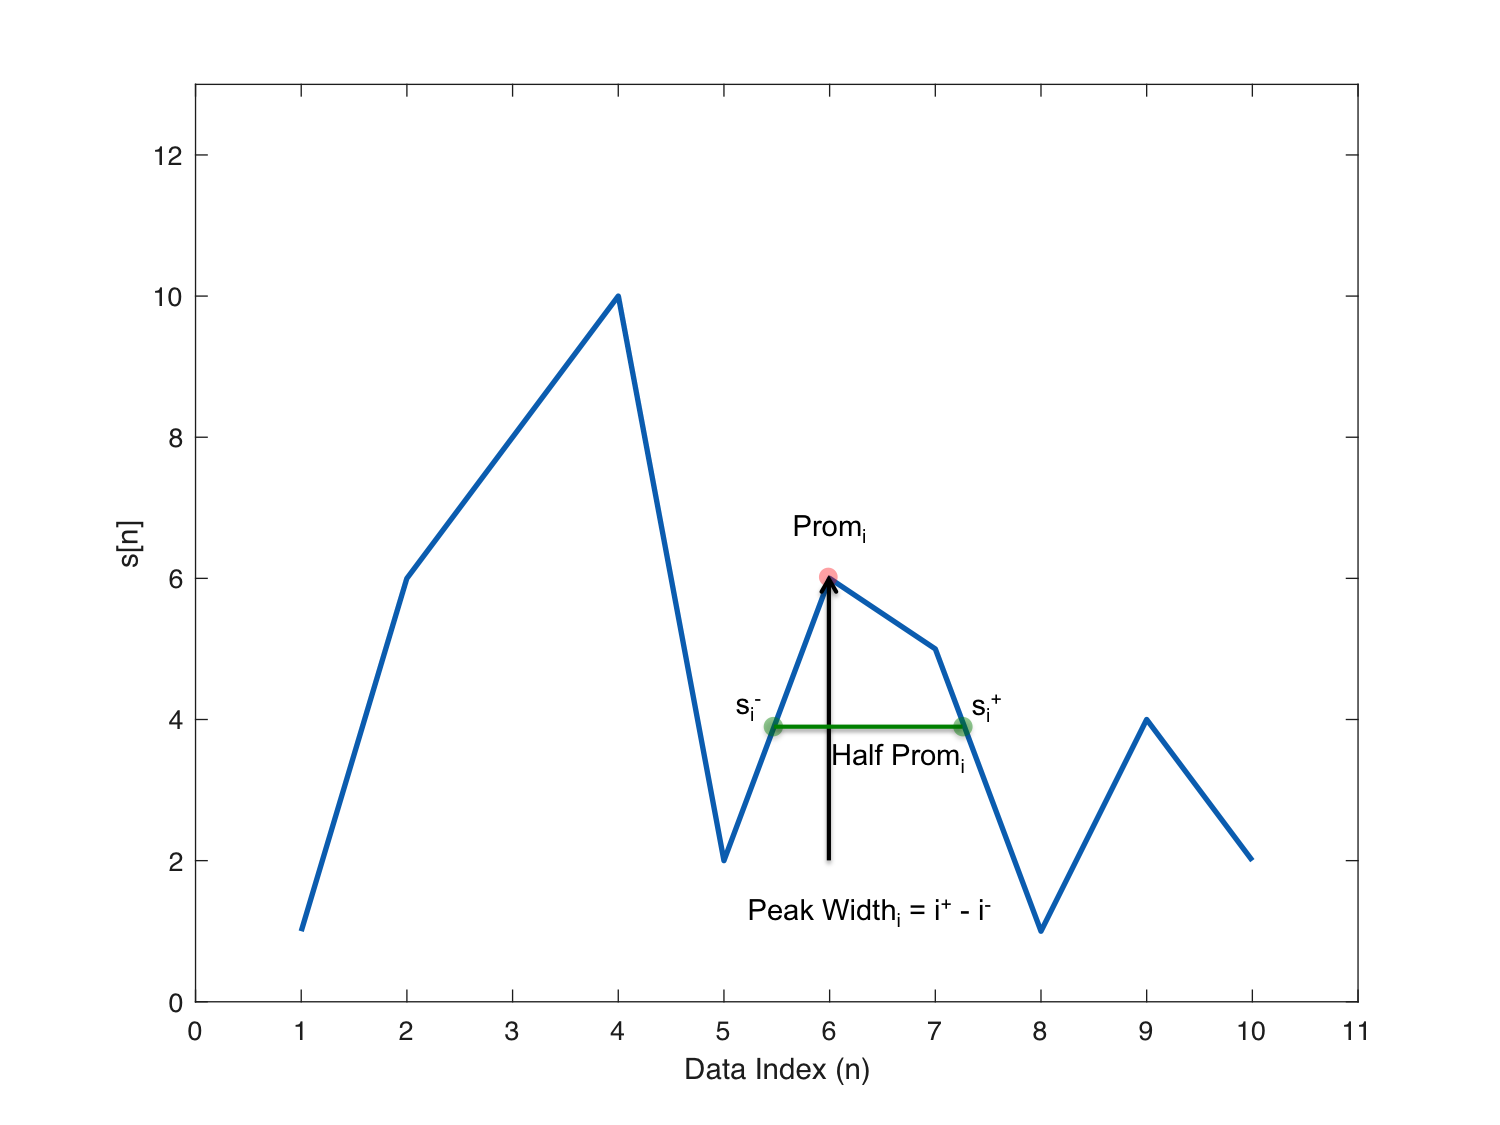
\includegraphics[width=7cm]{peakWidth}
    \medskip
    \centerline{(d)}
  \end{minipage}
	\caption{Algorithmic progression for calculating prominence and peak width at the point of half-prominence}
	\label{fig:algProg}
\end{figure}

\section{Results}
\label{sec:results}

\subsection{Screening Design of Experiments}
\label{ssec:doe}
The resonant response of acoustophoretic microfluidic devices has been shown to be non-linear and discontinuous \cite{garofalo2016performance}. Complex response patterns with numerous explanatory variables have been successfully optimized using a fractional factorial experimental design approach in conjunction with a response surface methodology (RSM) \cite{muriithi2015application}; however, these methodologies assume that the function $f(x)$ modeling the response variable $y$ to the explanatory variables $x=(x_1,x_2,\dots,x_n)$ accounting for some experimental error $\epsilon$, as shown in Equation \ref{eqn:response}, is a low-degree polynomial \cite{khuri2010response}. 

\begin{equation}
\label{eqn:response}
  \hfill y=f(x)+\epsilon \hfill
\end{equation}

In the absence of a near-quadratic response, multiple rounds of experiments are required to adequately detect a positive gradient in performance \cite{carley2004response}. Even after multiple rounds of experiments, the nature of a complex response surface means that no claim of optimality can be made \cite{box2006improving}. Since this study seeks a performance enhancement, as opposed to an optimal geometry, this iterative method is acceptable. 

Experiments must be initialized such that the sampling of the solution space can detect curvature in the response, as described in Section \ref{ssec:seeding}. Curvature in the response surface for an explanatory variable implies the existence of a local maxima in performance. Driving the design towards that local maxima is accomplished by isolating the variable in question and conducting experiments at adjacent points on the response plane, as outlined in Section \ref{ssec:iso}. 

Figure \ref{fig:geometry} illustrates the explanatory variables studied. Channel Width ($W_c$), channel height ($H_c$), side-wall width ($W_s$) and the position of the channel on the $y$-axis in two dimensional space ($Y_{pos}$) were selected as variables to study because they account for a majority of the two-dimensional design-space and are simple to vary during fabrication.


\subsection{Seeding of the Design Space}
\label{ssec:seeding}
In order to economize the number of initial experimental runs, an orthogonal array was chosen in order to generate a useful parameter set for the initial iteration of experiments. Orthogonal arrays are are used in design optimization to provide the most coverage of the solution space while minimizing the number of experimental runs \cite{yokoyama1993taguchi}. This is accomplished through the creation of an experimental set such that each combination of the array's strength appears equally often \cite{hedayat2012orthogonal}. The orthogonal array used to seed the design space is known as the $L_9 (3^4)$ array, which has a strength of two and is used to probe a solution space consisting of four explanatory variables at three settings in nine experimental runs, as opposed to the 81 experimental runs required to conduct the full-factorial experiment \cite{ting2004preparation}. The use of three explanatory variable settings was chosen in order to detect curvature in the response surface. The parameter set tested while seeding the design space, in accordance with an $L_9 (3^4)$ orthogonal array, is shown in Table \ref{tab:geometries}.

Since the parameters generated during the initial seeding of the design space cannot assume a functional geometry (i.e., a geometry capable of focusing blood), the purpose of the initial iteration of experiments is directed towards discovering functional designs, as opposed to a comparison between functional designs. As such, the performance parameter used during this initial phase is peak prominence (Figure \ref{fig:algProg}c.). This is because $\chi$ (Figure \ref{fig:algProg}d.) can skew the results by rewarding peaks with small prominence values (i.e., poor focusing) and correspondingly small widths.  
\begin{table}[h]
% table caption is above the table
	\caption[Geometries tested for L9 design array]{Geometries tested for L9 design array. All dimensions are given in units of $\mu$m. Prominence values are given in units of pixel intensity}
\label{tab:geometries}       % Give a unique label
% For LaTeX tables use
\centering
\begin{tabular}{llll|cc}
\hline\noalign{\smallskip}
$W_c$ & $H_c$ & $W_s$ & $Y_{Pos}$ & Prominence & Freq (MHz) \\
\noalign{\smallskip}\hline\noalign{\smallskip}
300 & 75 & 500 & Low & 6375 & 1.58\\
300 & 290 & 850 & Center & 5496 & 1.22\\
300 & 500 & 1200 & High & 8240 & 0.67\\
650 & 75 & 850 & High & 43021 & 0.55\\
650 & 290 & 1200 & Low & 12950 & 0.66\\
650 & 500 & 500 & Center & 13251 & 0.57\\
1000 & 75 & 1200 & Center & 14215 & 0.74\\
1000 & 290 & 500 & High & 9574 & 0.73\\
1000 & 500 & 850 & Low & 3144 & 0.71\\
\noalign{\smallskip}\hline
\end{tabular}
\end{table}
The response surface generated from the data points shown in Table \ref{tab:geometries} was analyzed using statistical software (JMP®, Version 13.0.0. SAS Institute Inc., Cary, NC, 1989-2017) and is shown in Figure \ref{fig:L9}. Maximum desirability of the performance parameter is achieved by setting $W_c$ to 650 $\mu$m, $H_c$ to 75$\mu$m, $W_s$ to 850 $\mu$m and placing the channel in the high vertical position. Additionally, the response surface shows significant curvature while modulating the width of the channel, leading into the next iteration of the study outlined in Section \ref{sssec:width}.

\begin{figure}[htb]
  \begin{minipage}[t]{0.99\linewidth}\centering
    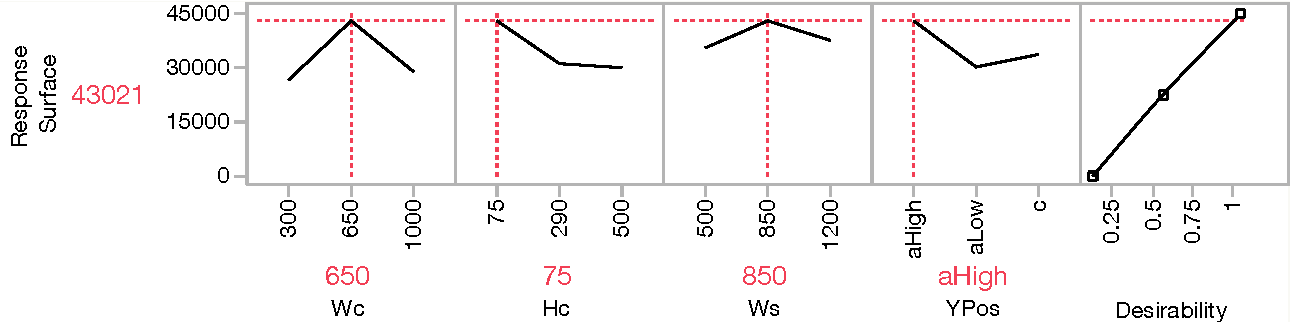
\includegraphics[width=14cm]{L9}
  \end{minipage}\hfill
  \caption[Results of initial seeding of design space]{Results of initial experimental run. The response surface is determined through a least squares fit of the prominence data shown in Table \ref{tab:geometries} in four-dimensional space.}
	\label{fig:L9}
\end{figure}

\subsection{Variable Isolation Studies}
\label{ssec:iso}

\subsubsection{Channel Width Study}
\label{sssec:width}

Difficulties manufacturing chips with $H_c$ of 75 $\mu$m, namely the total collapse of the channel during bonding, resulted in an increase of $H_c$ from 75 $\mu$m to 100 $\mu$m for the subsequent variable isolation study; the assumption being that such a small change to the height of the channel would not result in a large change in performance. However, Tables \ref{tab:geometries} and \ref{tab:width} show a significant performance degradation as a result of the change for the designs having a channel width of 650 $\mu$m. As all other parameters were held constant, it can be assumed that the performance degradation is a result of increasing the channel height from 75 $\mu$m to 100 $\mu$m. 

\begin{table}[h]
% table caption is above the table
	\caption[Geometries tested for an isolation study of channel width]{Geometries tested for an isolation study of channel width. All dimensions are given in units of $\mu$m. The frequency range scanned spanned from 500 kHz to 2 MHz. No fundamental odd mode was observed within this range for the design with a channel width of 700 $\mu$m.}
\label{tab:width}       % Give a unique label
% For LaTeX tables use
\centering
\begin{tabular}{llll|cc}
\hline\noalign{\smallskip}
$W_c$ & $H_c$ & $W_s$ & $Y_{Pos}$ & Prominence & Freq (MHz)\\
\noalign{\smallskip}\hline\noalign{\smallskip}
500 & 100 & 850 & High & 12143 & 0.64\\
550 & 100 & 850 & High & 15200 & 0.51\\
600 & 100 & 850 & High & 4770 & 1.58\\
650 & 100 & 850 & High & 5470 & 1.99\\
700 & 100 & 850 & High & - & - \\
\noalign{\smallskip}\hline
\end{tabular}
\end{table}

As shown in Table \ref{tab:width}, the highest performing channel width, holding other factors constant, was 550 $\mu$m. As a significant performance shift was observed as a result of a small adjustment to $H_c$, channel height was chosen as the variable to isolate for the final screening assay.

\subsubsection{Channel Height Study}
\label{sssec:height}

The final screening assay, as specified in Section \ref{sssec:finalScreen}, was conducted by fixing $W_c$, $W_s$, and $Y_{Pos}$ while varying $H_c$. The geometries studied are shown in Table \ref{tab:height}. The results shown in Figure \ref{fig:heightPlot} demonstrate that, for flow rates higher than 25 $\mu$l/min, the chip with a channel height of 250 $\mu$m performed better than the other chips tested in terms of $\chi$ at all studied power levels. Thus the winning geometry of the study's device screening stage has a channel width of 550 $\mu$m, a channel height of 250 $\mu$m, a side-wall width of 850 $\mu$m, with the channel in the High vertical position.

\begin{table}[h]
% table caption is above the table
	\caption[Geometries tested for an isolation study of channel height]{Geometries tested for an isolation study of channel height. All dimensions are given in units of $\mu$m.}
\label{tab:height}       % Give a unique label
% For LaTeX tables use
\centering
\begin{tabular}{llll}
\hline\noalign{\smallskip}
$W_c$ & $H_c$ & $W_s$ & $Y_{Pos}$ \\
\noalign{\smallskip}\hline\noalign{\smallskip}
550 & 100 & 850 & High\\
550 & 150 & 850 & High\\
550 & 200 & 850 & High\\
550 & 250 & 850 & High\\
550 & 300 & 850 & High\\
\noalign{\smallskip}\hline
\end{tabular}
\end{table}

\begin{figure}[H]
  \begin{minipage}[t]{0.49\linewidth}\centering
    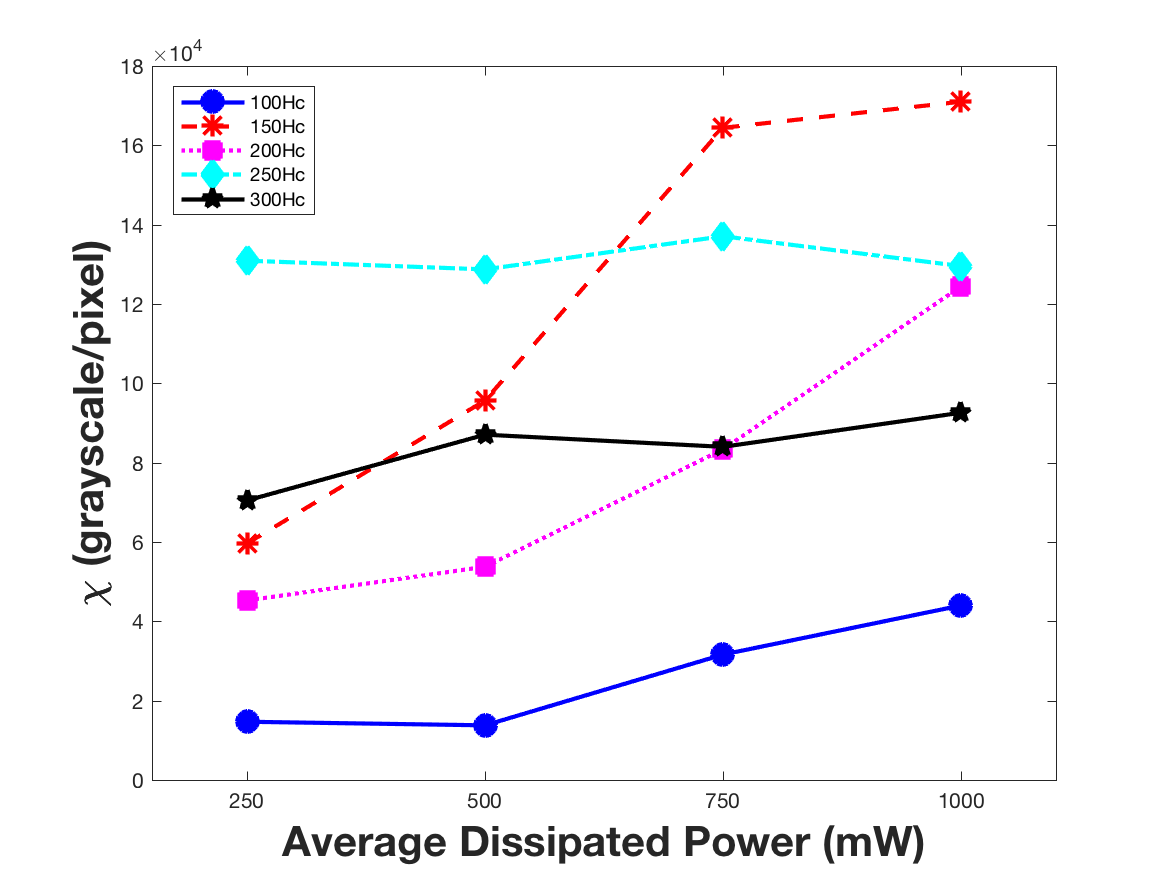
\includegraphics[width=7cm]{HeightPlot25ul}
    \medskip
    \centerline{(a)}
  \end{minipage}\hfill
  \begin{minipage}[t]{0.49\linewidth}\centering
    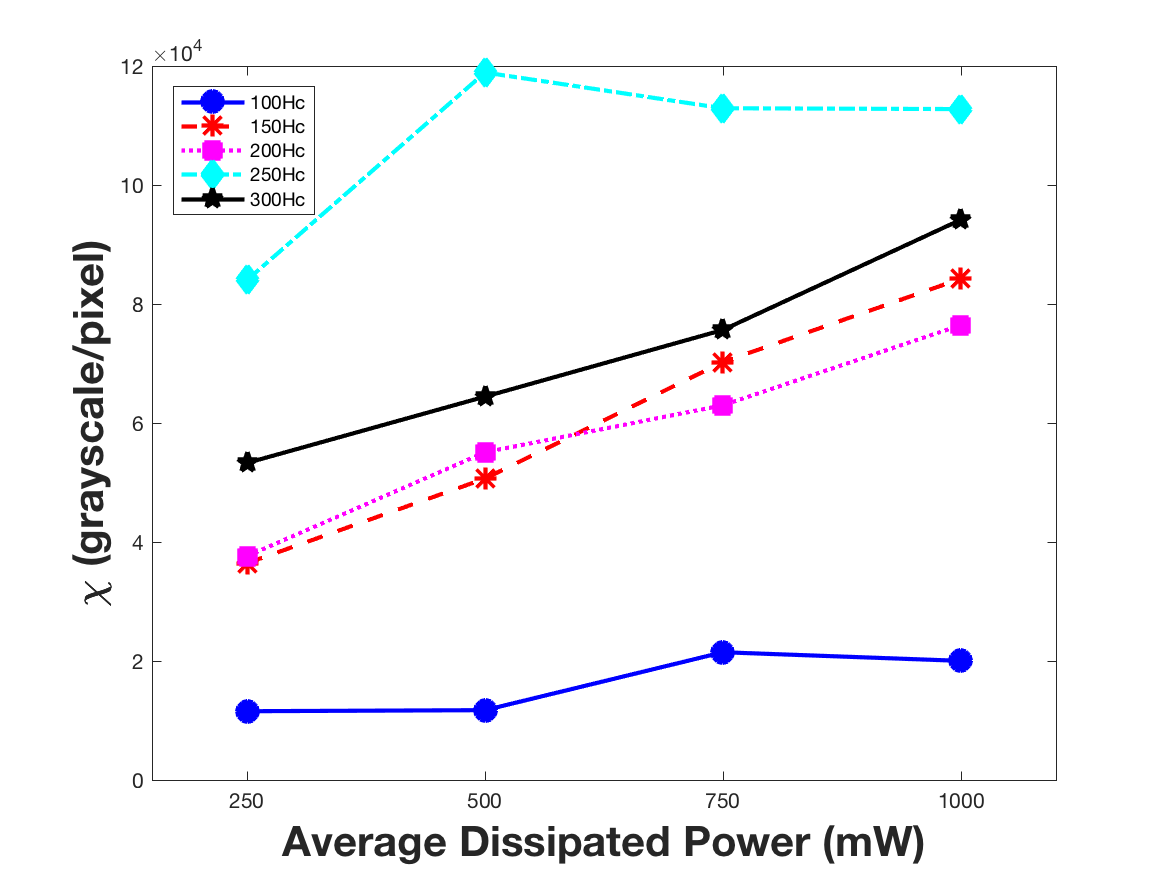
\includegraphics[width=7cm]{HeightPlot50ul}
    \medskip
    \centerline{(b)}\\
  \end{minipage}
  \begin{minipage}[t]{0.99\linewidth}\centering
    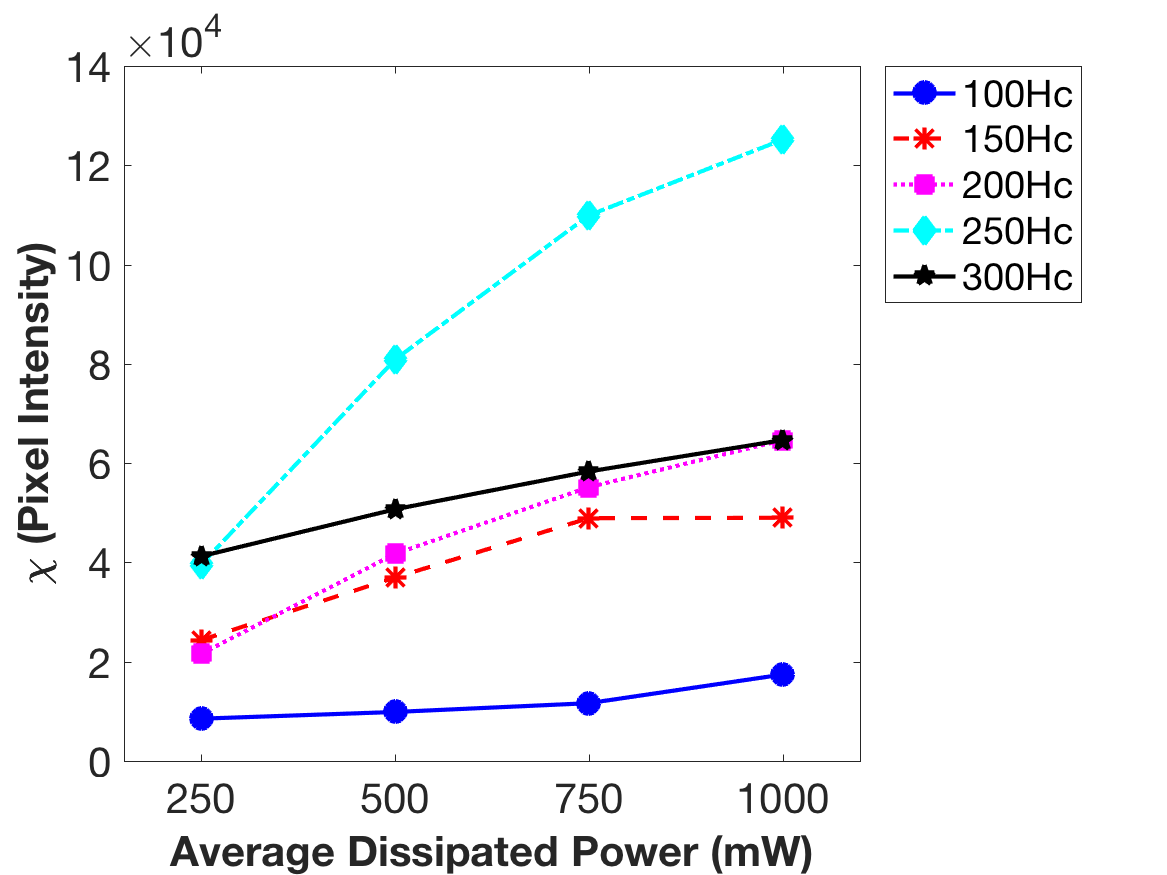
\includegraphics[width=7cm]{HeightPlot75ul}
    \medskip
    \centerline{(c)}
  \end{minipage}
  \caption[Performance Comparison of Channel Height Study using Image Analysis]{Performance Comparison of Channel Height Study using Image Analysis. (a-c) plot the performance of the geometries in Table \ref{tab:height} for three volumetric flow rates: 25 $\mu$l/m, 50 $\mu$l/m and 75 $\mu$l/m, respectively. Performance is calculated from microscope images in the manner described in Section \ref{ssec:promToWidth}.}
	\label{fig:heightPlot}
\end{figure}


\subsection{Comparison of Winning Geometry versus Baseline Geometry}
\label{ssec:comparison}

The results of the screening assays yielded a geometry that outperformed the other devices under test. However, in order to gauge the ultimate success of this geometry it must be tested against the baseline geometry. This section presents results from three experiments that compared the winning geometry of the screening assays against the baseline geometry through image analysis, blood separation, and bacteria separation.


\subsubsection{Comparative Focusing}
\label{sssec:comparisonFocusing}

Figure \ref{fig:headToHeadImages}(a--c) plots the performance of the winning geometry, hereafter referred to as Chip 2.0, against the baseline in terms $\chi$. The results show that Chip 2.0 outperforms the baseline for all tested combinations of flow and power settings.

\begin{figure}[H]
  \begin{minipage}[t]{0.49\linewidth}\centering
    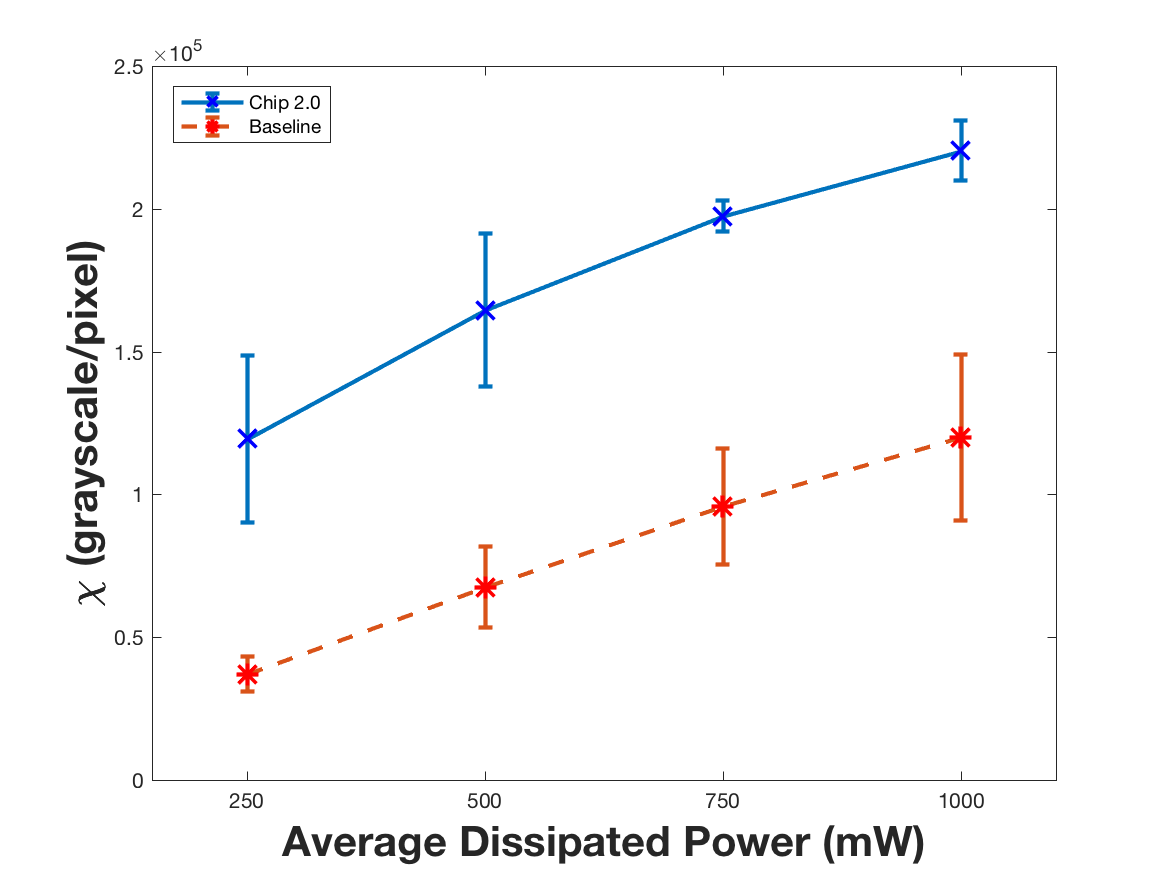
\includegraphics[width=7cm]{ErrorBars25ul}
    \medskip
    \centerline{(a)}
  \end{minipage}\hfill
  \begin{minipage}[t]{0.49\linewidth}\centering
    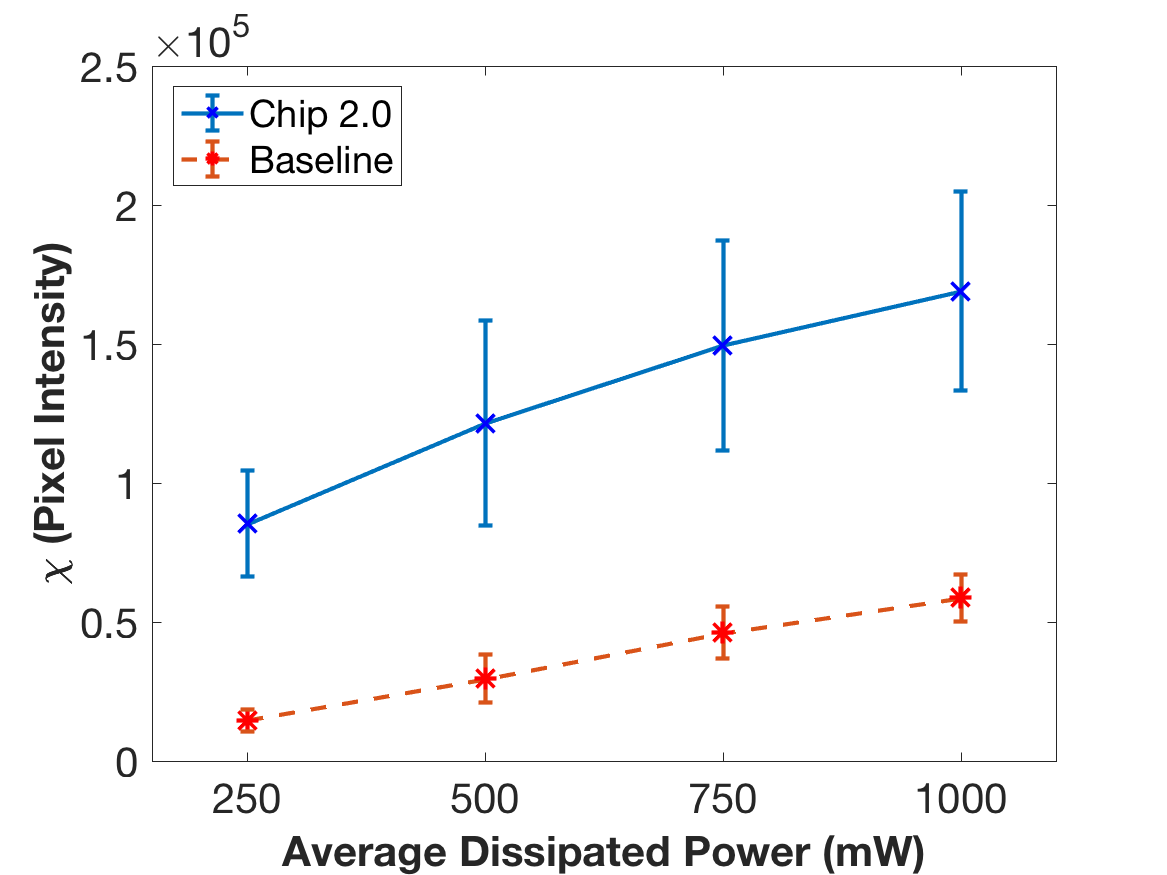
\includegraphics[width=7cm]{ErrorBars50ul}
    \medskip
    \centerline{(b)}\\
  \end{minipage}
  \begin{minipage}[t]{0.99\linewidth}\centering
    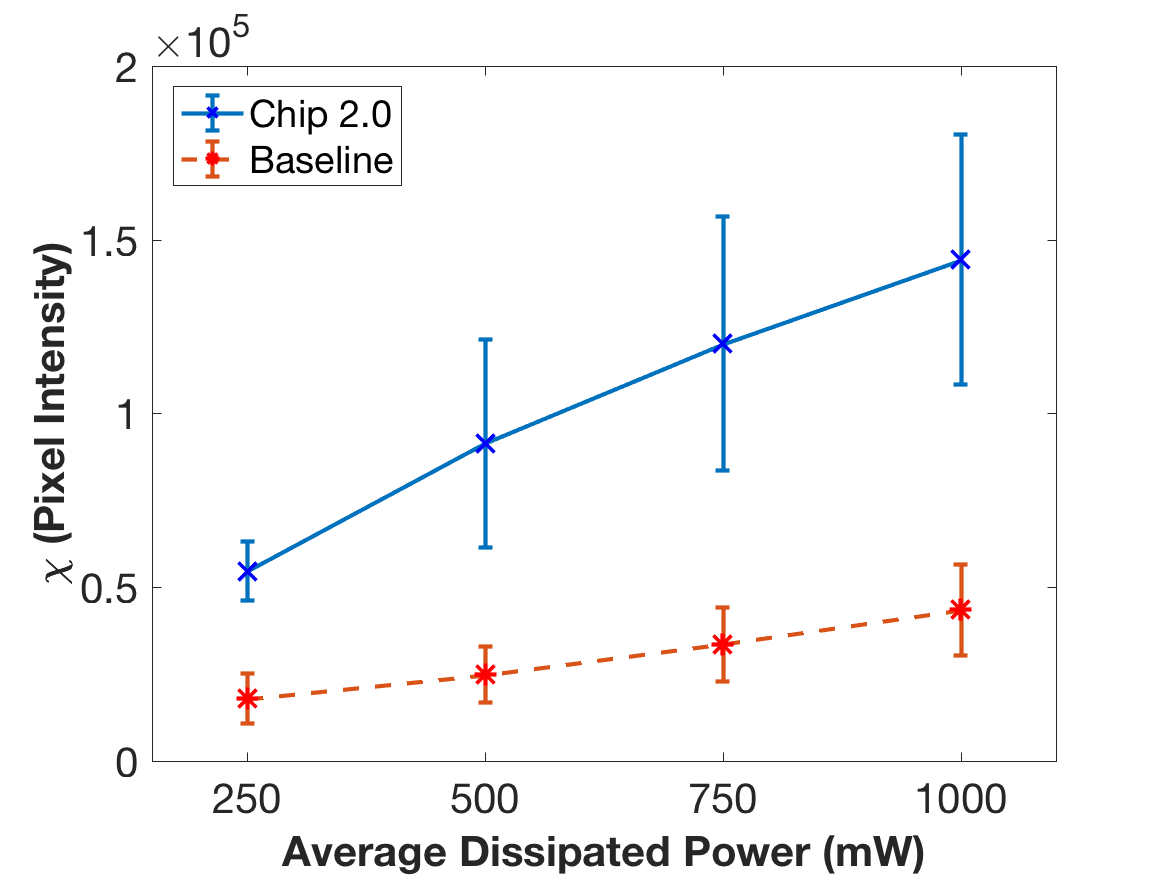
\includegraphics[width=7cm]{ErrorBars75ul}
    \medskip
    \centerline{(c)}
  \end{minipage}
  \caption[Performance Comparison Versus Baseline using Image Analysis]{Performance Comparison Versus Baseline using Image Analysis. (a-c) plot the performance of the baseline versus the winner of the study for three volumetric flow rates: 25 $\mu$l/m, 50 $\mu$l/m and 75 $\mu$l/m, respectively. Performance is calculated from microscope images in the manner described in Section \ref{ssec:promToWidth}.}
	\label{fig:headToHeadImages}
\end{figure}

\subsubsection{Comparative Blood Separation}
\label{sssec:comparisonBlood}

Figure \ref{fig:headToHeadBlood} plots the performance of Chip 2.0 against the baseline in terms of each device's ability to focus RBCs to the center port. The dynamic range of each measurement was limited to that which falls between the performance at the control measurement (i.e., zero average dissipated power) and 100\% RBC concentration in the center channel. As the chip design used, shown in Figure \ref{fig:geometry}, has a single input port and two outlet ports, RBCs will be equally distributed between the two outlet ports in the acoustics-off (0 W input power) condition. The baseline and Chip 2.0 demonstrated comparable performance at a flow rate of 25 $\mu$l/min across all power settings; however, at higher flow rates Chip 2.0 outperformed the baseline across all non-control power settings. \textbf{How can I quantify the percent change in performance across all experimental conditions?}.

\begin{figure}[H]
  \begin{minipage}[t]{0.49\linewidth}\centering
    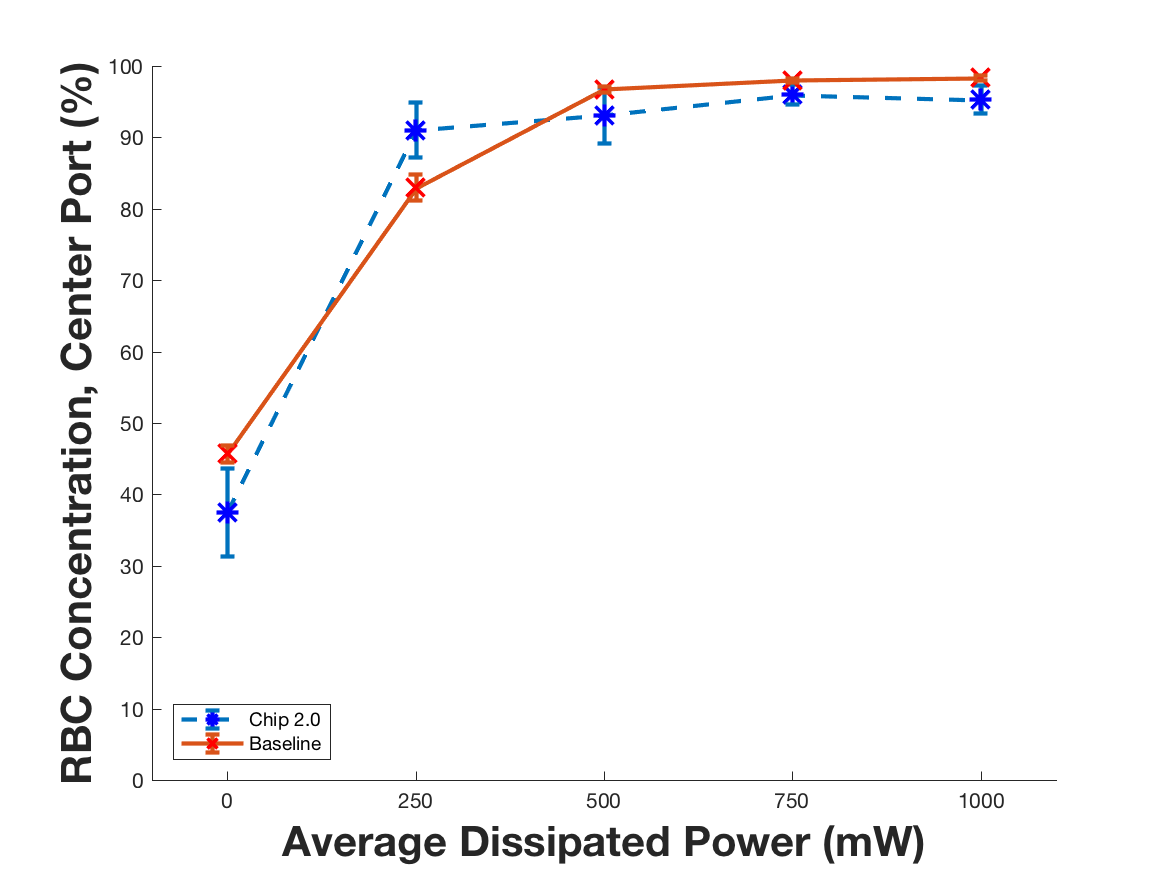
\includegraphics[width=7cm]{ErrorBarBloodData25ul}
    \medskip
    \centerline{(a)}
  \end{minipage}\hfill
  \begin{minipage}[t]{0.49\linewidth}\centering
    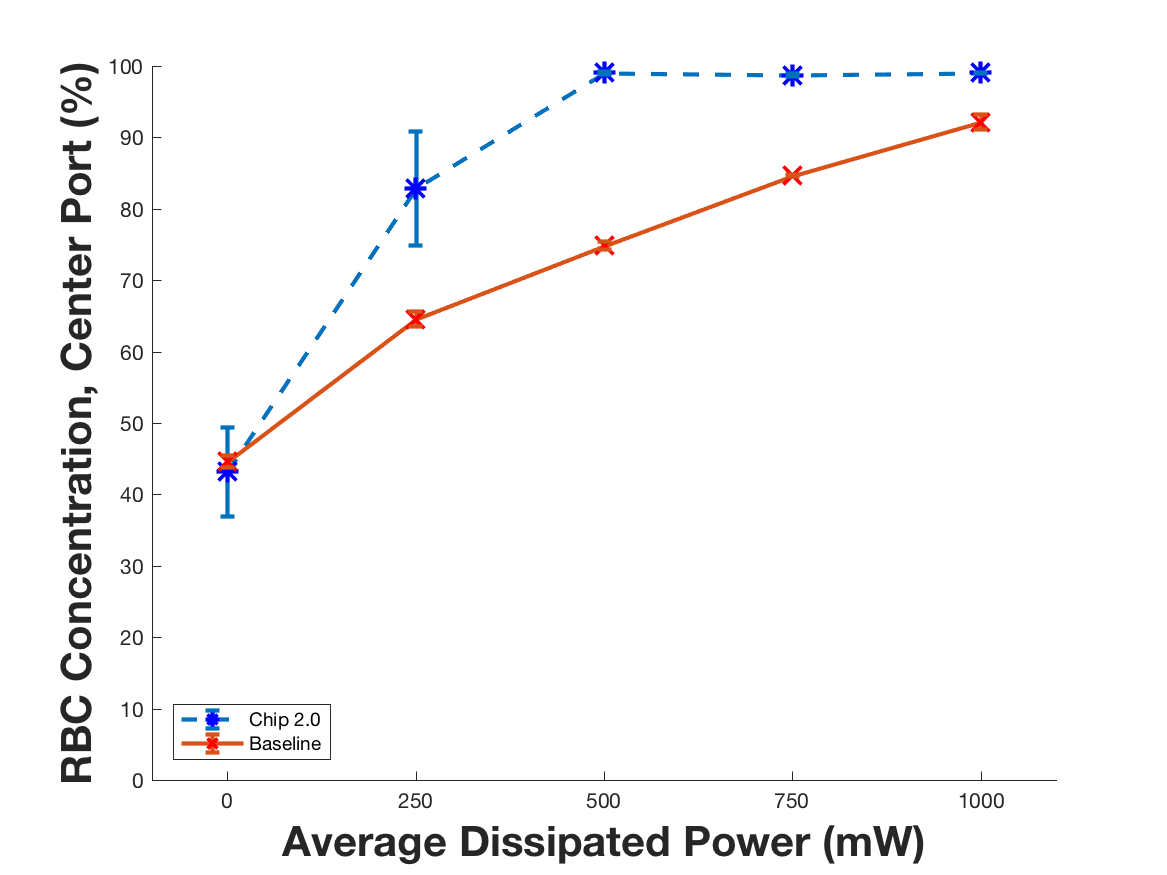
\includegraphics[width=7cm]{ErrorBarBloodData50ul}
    \medskip
    \centerline{(b)}\\
  \end{minipage}
  \begin{minipage}[t]{0.99\linewidth}\centering
    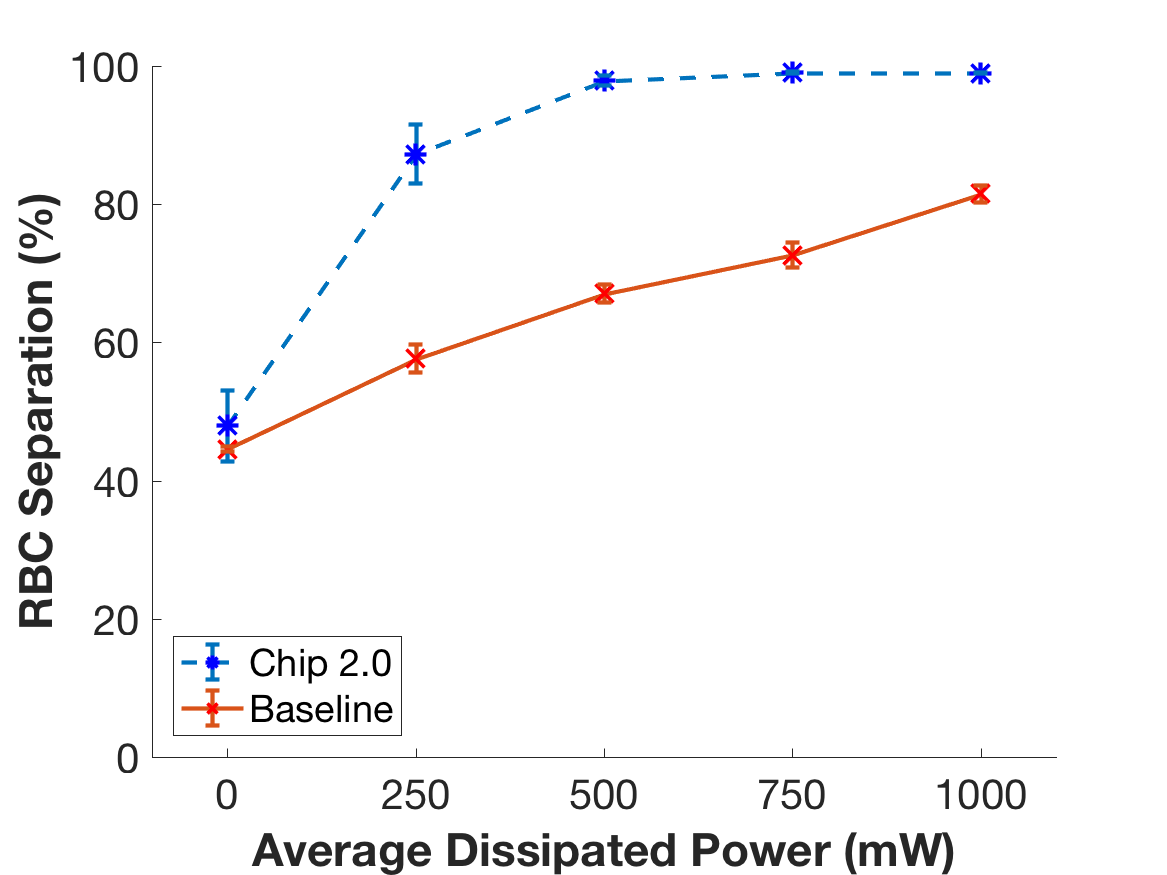
\includegraphics[width=7cm]{ErrorBarBloodData75ul}
    \medskip
    \centerline{(c)}
  \end{minipage}
  \caption[Separation Performance Comparison Versus Baseline]{Separation Performance Comparison Versus Baseline. (a-c) plot the performance of the baseline versus the winner of the study for three volumetric flow rates: 25 $\mu$l/m, 50 $\mu$l/m and 75 $\mu$l/m, respectively. Performance is defined based on each design's ability to focus red blood cells into the middle channel of the trifurcation shown in Figure \ref{fig:geometry}.}
	\label{fig:headToHeadBlood}
\end{figure}

\subsubsection{Comparative Bacterial Separation}
\label{sssec:comparisonBacteria}

\textbf{TODO Parker: Please populate this section with the results of the plating experiment. We can work together on the discussion}

\section{Conclusion}
\label{sec:conclusion}

The results of the comparison experiments show that Chip 2.0 improves performance relative to the baseline geometry by \textbf{XXX}\% across all three metrics: focusing, blood separation and bacterial separation.


